\documentclass[twoside]{book}

% Packages required by doxygen
\usepackage{calc}
\usepackage{doxygen}
\usepackage{graphicx}
\usepackage[utf8]{inputenc}
\usepackage{makeidx}
\usepackage{multicol}
\usepackage{multirow}
\usepackage{textcomp}
\usepackage[table]{xcolor}

% Font selection
\usepackage[T1]{fontenc}
\usepackage{mathptmx}
\usepackage[scaled=.90]{helvet}
\usepackage{courier}
\usepackage{amssymb}
\usepackage{sectsty}
\renewcommand{\familydefault}{\sfdefault}
\allsectionsfont{%
  \fontseries{bc}\selectfont%
  \color{darkgray}%
}
\renewcommand{\DoxyLabelFont}{%
  \fontseries{bc}\selectfont%
  \color{darkgray}%
}

% Page & text layout
\usepackage{geometry}
\geometry{%
  a4paper,%
  top=2.5cm,%
  bottom=2.5cm,%
  left=2.5cm,%
  right=2.5cm%
}
\tolerance=750
\hfuzz=15pt
\hbadness=750
\setlength{\emergencystretch}{15pt}
\setlength{\parindent}{0cm}
\setlength{\parskip}{0.2cm}
\makeatletter
\renewcommand{\paragraph}{%
  \@startsection{paragraph}{4}{0ex}{-1.0ex}{1.0ex}{%
    \normalfont\normalsize\bfseries\SS@parafont%
  }%
}
\renewcommand{\subparagraph}{%
  \@startsection{subparagraph}{5}{0ex}{-1.0ex}{1.0ex}{%
    \normalfont\normalsize\bfseries\SS@subparafont%
  }%
}
\makeatother

% Headers & footers
\usepackage{fancyhdr}
\pagestyle{fancyplain}
\fancyhead[LE]{\fancyplain{}{\bfseries\thepage}}
\fancyhead[CE]{\fancyplain{}{}}
\fancyhead[RE]{\fancyplain{}{\bfseries\leftmark}}
\fancyhead[LO]{\fancyplain{}{\bfseries\rightmark}}
\fancyhead[CO]{\fancyplain{}{}}
\fancyhead[RO]{\fancyplain{}{\bfseries\thepage}}
\fancyfoot[LE]{\fancyplain{}{}}
\fancyfoot[CE]{\fancyplain{}{}}
\fancyfoot[RE]{\fancyplain{}{\bfseries\scriptsize Generated on Tue Feb 26 2019 15\-:54\-:55 for Molssi Driver Interface Library by Doxygen }}
\fancyfoot[LO]{\fancyplain{}{\bfseries\scriptsize Generated on Tue Feb 26 2019 15\-:54\-:55 for Molssi Driver Interface Library by Doxygen }}
\fancyfoot[CO]{\fancyplain{}{}}
\fancyfoot[RO]{\fancyplain{}{}}
\renewcommand{\footrulewidth}{0.4pt}
\renewcommand{\chaptermark}[1]{%
  \markboth{#1}{}%
}
\renewcommand{\sectionmark}[1]{%
  \markright{\thesection\ #1}%
}

% Indices & bibliography
\usepackage{natbib}
\usepackage[titles]{tocloft}
\setcounter{tocdepth}{3}
\setcounter{secnumdepth}{5}
\makeindex

% Hyperlinks (required, but should be loaded last)
\usepackage{ifpdf}
\ifpdf
  \usepackage[pdftex,pagebackref=true]{hyperref}
\else
  \usepackage[ps2pdf,pagebackref=true]{hyperref}
\fi
\hypersetup{%
  colorlinks=true,%
  linkcolor=blue,%
  citecolor=blue,%
  unicode%
}

% Custom commands
\newcommand{\clearemptydoublepage}{%
  \newpage{\pagestyle{empty}\cleardoublepage}%
}


%===== C O N T E N T S =====

\begin{document}

% Titlepage & ToC
\hypersetup{pageanchor=false}
\pagenumbering{roman}
\begin{titlepage}
\vspace*{7cm}
\begin{center}%
{\Large Molssi Driver Interface Library }\\
\vspace*{1cm}
{\large Generated by Doxygen 1.8.5}\\
\vspace*{0.5cm}
{\small Tue Feb 26 2019 15:54:55}\\
\end{center}
\end{titlepage}
\clearemptydoublepage
\tableofcontents
\clearemptydoublepage
\pagenumbering{arabic}
\hypersetup{pageanchor=true}

%--- Begin generated contents ---
\chapter{Main Page}
\label{index}\hypertarget{index}{}\hypertarget{index_overview_sec}{}\section{Overview}\label{index_overview_sec}
The Mol\-S\-S\-I Driver Interface (M\-D\-I) library enables codes to interoperate via the M\-D\-I.\hypertarget{index_source_sec}{}\section{Source Code}\label{index_source_sec}
The source code of the M\-D\-I library is available at Git\-Hub at \href{https://github.com/MolSSI/molssi_driver_interface}{\tt https\-://github.\-com/\-Mol\-S\-S\-I/molssi\-\_\-driver\-\_\-interface}\hypertarget{index_commands_sec}{}\section{M\-D\-I Standard}\label{index_commands_sec}
\hypertarget{index_initialization_options}{}\subsection{M\-D\-I Initialization Options}\label{index_initialization_options}
\begin{DoxyParagraph}{}
{\bfseries  -\/role\-: } The role of this code in the context of M\-D\-I communication. Valid arguments are D\-R\-I\-V\-E\-R and E\-N\-G\-I\-N\-E \par
 {\bfseries  -\/name\-: } A short string that identifies this code. See the {\ttfamily $<$N\-A\-M\-E} command for more information. \par
 {\bfseries  -\/method\-: } The method by which M\-D\-I will handle communication between the codes. Valid arguments are M\-P\-I and T\-C\-P. \par
 {\bfseries  -\/hostname\-: } For E\-N\-G\-I\-N\-E\-S, when using the T\-C\-P communication method, specifies the hostname of the driver. \par
 {\bfseries  -\/port\-: } When using the T\-C\-P communication method, specifies the port at which the driver will listen for incoming connections.
\end{DoxyParagraph}
\hypertarget{index_command_list}{}\subsection{Command List}\label{index_command_list}
The following is a list of commands that are officially part of the M\-D\-I standard.

All physical quantities communicated through M\-D\-I must be expressed in atomic units.\hypertarget{index_atomic_step}{}\subsubsection{A\-T\-O\-M\-\_\-\-S\-T\-E\-P}\label{index_atomic_step}
The engine performs a time propagation step for the atomic coordinates. The engine updates its energy, which can be queried with the {\ttfamily $<$E\-N\-E\-R\-G\-Y} command.\hypertarget{index_set_cell}{}\subsubsection{$>$\-C\-E\-L\-L}\label{index_set_cell}
The driver sends a set of cell vectors to the engine, which resizes its simulation cell to the dimensions specified by the cell vectors.

\begin{DoxyParagraph}{}
{\bfseries  Data Type\-: } M\-D\-I\-\_\-\-D\-O\-U\-B\-L\-E \par
 {\bfseries  Quantity\-: } 9 \par
 {\bfseries  Injection\-: } Immediate \par
 {\bfseries  Note\-: } In the case of a quantum chemistry code that uses a plane wave basis set, the engine will recalculate the g-\/vectors either immediately or at the beginning of the next S\-C\-F command.
\end{DoxyParagraph}
\hypertarget{index_recv_cell}{}\subsubsection{$<$\-C\-E\-L\-L}\label{index_recv_cell}
The engine sends a set of cell vectors to the driver, in the same format as specified for the {\ttfamily $>$C\-E\-L\-L} command.

\begin{DoxyParagraph}{}
{\bfseries  Data Type\-: } M\-D\-I\-\_\-\-D\-O\-U\-B\-L\-E \par
 {\bfseries  Quantity\-: } 9
\end{DoxyParagraph}
\hypertarget{index_send_charges}{}\subsubsection{$>$\-C\-H\-A\-R\-G\-E\-S}\label{index_send_charges}
The driver sends a set of atomic charges to the engine, which replaces its atomic charges with those sent by the driver.

\begin{DoxyParagraph}{}
{\bfseries  Data Type\-: } M\-D\-I\-\_\-\-D\-O\-U\-B\-L\-E \par
 {\bfseries  Quantity\-: } {\ttfamily $<$N\-A\-T\-O\-M\-S} \par
 {\bfseries  Format\-: } Sequentially ascending order of atomic index \par
 {\bfseries  Injection\-: } Immediate \par

\end{DoxyParagraph}
\hypertarget{index_recv_charges}{}\subsubsection{$<$\-C\-H\-A\-R\-G\-E\-S}\label{index_recv_charges}
The engine sends a set of atomic charges to the driver, in the same format as specified for the {\ttfamily $>$C\-H\-A\-R\-G\-E\-S} command.

\begin{DoxyParagraph}{}
{\bfseries  Data Type\-: } M\-D\-I\-\_\-\-D\-O\-U\-B\-L\-E \par
 {\bfseries  Quantity\-: } {\ttfamily $<$N\-A\-T\-O\-M\-S} \par
 {\bfseries  Format\-: } Sequentially ascending order of atomic index
\end{DoxyParagraph}
\hypertarget{index_send_coords}{}\subsubsection{$>$\-C\-O\-O\-R\-D\-S}\label{index_send_coords}
The driver sends a set of atomic coordinates to the engine, which replaces its atomic coordinates with those sent by the driver.

\begin{DoxyParagraph}{}
{\bfseries  Data Type\-: } M\-D\-I\-\_\-\-D\-O\-U\-B\-L\-E \par
 {\bfseries  Quantity\-: } {\ttfamily  3 $\ast$ $<$N\-A\-T\-O\-M\-S } \par
 {\bfseries  Format\-: } Sequentially ascending order of atomic index, with the coordinates for each individual atom being provided in xyz order \par
 {\bfseries  Injection\-: } Immediate
\end{DoxyParagraph}
\hypertarget{index_recv_coords}{}\subsubsection{$<$\-C\-O\-O\-R\-D\-S}\label{index_recv_coords}
The engine sends a set of atomic coordinates to the driver.

\begin{DoxyParagraph}{}
{\bfseries  Data Type\-: } M\-D\-I\-\_\-\-D\-O\-U\-B\-L\-E \par
 {\bfseries  Quantity\-: } {\ttfamily  3 $\ast$ $<$N\-A\-T\-O\-M\-S } \par
 {\bfseries  Format\-: } Sequentially ascending order of atomic index, with the coordinates for each individual atom being provided in xyz order
\end{DoxyParagraph}
\hypertarget{index_recv_energy}{}\subsubsection{$<$\-E\-N\-E\-R\-G\-Y}\label{index_recv_energy}
The engine sends its most recently calculated energy to the driver. The {\ttfamily M\-D\-\_\-\-I\-N\-I\-T}, {\ttfamily S\-C\-F}, and {\ttfamily A\-T\-O\-M\-\_\-\-S\-T\-E\-P} commands can be used to cause the engine to calculate a new energy.

\begin{DoxyParagraph}{}
{\bfseries  Data Type\-: } M\-D\-I\-\_\-\-D\-O\-U\-B\-L\-E \par
 {\bfseries  Quantity\-: } 1
\end{DoxyParagraph}
\hypertarget{index_exit_command}{}\subsubsection{E\-X\-I\-T}\label{index_exit_command}
The engine terminates and can no longer be sent commands.\hypertarget{index_send_forces}{}\subsubsection{$>$\-F\-O\-R\-C\-E\-S}\label{index_send_forces}
The driver sends a set of atomic forces to the engine, which replaces its internal forces with the forces sent by the driver.

\begin{DoxyParagraph}{}
{\bfseries  Data Type\-: } M\-D\-I\-\_\-\-D\-O\-U\-B\-L\-E \par
 {\bfseries  Quantity\-: } {\ttfamily  3 $\ast$ $<$N\-A\-T\-O\-M\-S } \par
 {\bfseries  Format\-: } Sequentially ascending order of atomic index, with the forces for each individual atom being provided in xyz order \par
 {\bfseries  Injection\-: } In response to the {\ttfamily A\-T\-O\-M\-\_\-\-S\-T\-E\-P} command, after any normal calculation of forces and immediately prior to propagation of the atomic positions
\end{DoxyParagraph}
\hypertarget{index_send_add_forces}{}\subsubsection{$>$+\-F\-O\-R\-C\-E\-S}\label{index_send_add_forces}
The driver sends a set of atomic forces to the engine, which adds the forces sent by the driver to its internal forces.

\begin{DoxyParagraph}{}
{\bfseries  Data Type\-: } M\-D\-I\-\_\-\-D\-O\-U\-B\-L\-E \par
 {\bfseries  Quantity\-: } {\ttfamily  3 $\ast$ $<$N\-A\-T\-O\-M\-S } \par
 {\bfseries  Format\-: } Sequentially ascending order of atomic index, with the forces for each individual atom being provided in xyz order \par
 {\bfseries  Injection\-: } In response to the {\ttfamily A\-T\-O\-M\-\_\-\-S\-T\-E\-P} command, after any normal calculation of forces and immediately prior to propagation of the atomic positions
\end{DoxyParagraph}
\hypertarget{index_recv_forces}{}\subsubsection{$<$\-F\-O\-R\-C\-E\-S}\label{index_recv_forces}
The engine calculates and sends a set of atomic forces to the driver. These forces include all force contributions, including the force contributions associated with any constraint algorithm (e.\-g. S\-H\-A\-K\-E, R\-A\-T\-T\-L\-E, etc.).

\begin{DoxyParagraph}{}
{\bfseries  Data Type\-: } M\-D\-I\-\_\-\-D\-O\-U\-B\-L\-E \par
 {\bfseries  Quantity\-: } {\ttfamily  3 $\ast$ $<$N\-A\-T\-O\-M\-S } \par
 {\bfseries  Format\-: } Sequentially ascending order of atomic index, with the forces for each individual atom being provided in xyz order
\end{DoxyParagraph}
\hypertarget{index_recv_masses}{}\subsubsection{$<$\-M\-A\-S\-S\-E\-S}\label{index_recv_masses}
The engine sends the driver the mass of each of the atom types.

\begin{DoxyParagraph}{}
{\bfseries  Data Type\-: } M\-D\-I\-\_\-\-D\-O\-U\-B\-L\-E \par
 {\bfseries  Quantity\-: } {\ttfamily  $<$N\-T\-Y\-P\-E\-S } \par
 {\bfseries  Format\-: } Sequentially ascending order of type index (see the {\ttfamily $<$T\-Y\-P\-E\-S} command)
\end{DoxyParagraph}
\hypertarget{index_md_init}{}\subsubsection{M\-D\-\_\-\-I\-N\-I\-T}\label{index_md_init}
The engine performs any initialization operations that are necessary before an M\-D simulation can be time propagated through the use of the {\ttfamily A\-T\-O\-M\-\_\-\-S\-T\-E\-P} command. This engine calculates the energy of the system, which can be queried by the {\ttfamily $<$E\-N\-E\-R\-G\-Y} command.

\begin{DoxyParagraph}{}
{\bfseries  Note\-: } This command may change the engine's atomic coordinates under certain circumstances, such as if the S\-H\-A\-K\-E algorithm is used.
\end{DoxyParagraph}
\hypertarget{index_send_name}{}\subsubsection{$<$\-N\-A\-M\-E}\label{index_send_name}
The engine sends the driver a string that corresponds to the argument of {\ttfamily -\/name} in the M\-D\-I initialization options. This argument allows a driver to identify the purpose of connected engine codes within the simulation. For example, a particular Q\-M/\-M\-M driver might require a connection with a single M\-M code and a single Q\-M code, with the expected name of the M\-M code being \char`\"{}\-M\-M\char`\"{} and the expected name of the Q\-M code being \char`\"{}\-Q\-M\char`\"{}. After initializing M\-D\-I and accepting communicators to the engines, the driver can use this command to identify which of the engines is the M\-M code and which is the Q\-M code.

\begin{DoxyParagraph}{}
{\bfseries  Data Type\-: } M\-D\-I\-\_\-\-C\-H\-A\-R \par
 {\bfseries  Quantity\-: } {\ttfamily  M\-D\-I\-\_\-\-N\-A\-M\-E\-\_\-\-L\-E\-N\-G\-T\-H }
\end{DoxyParagraph}
\hypertarget{index_recv_natoms}{}\subsubsection{$<$\-N\-A\-T\-O\-M\-S}\label{index_recv_natoms}
The engine sends the driver the number of atoms in the engine's system.

\begin{DoxyParagraph}{}
{\bfseries  Data Type\-: } M\-D\-I\-\_\-\-I\-N\-T \par
 {\bfseries  Quantity\-: } 1
\end{DoxyParagraph}
\hypertarget{index_recv_types}{}\subsubsection{$<$\-N\-T\-Y\-P\-E\-S}\label{index_recv_types}
The engine sends the driver the number of different types of atoms (e.\-g. \char`\"{}\-H\char`\"{}, \char`\"{}\-He\char`\"{}, \char`\"{}\-C\char`\"{}, \char`\"{}\-O\char`\"{}, etc.) in the engine's system.

\begin{DoxyParagraph}{}
{\bfseries  Data Type\-: } M\-D\-I\-\_\-\-I\-N\-T \par
 {\bfseries  Quantity\-: } 1
\end{DoxyParagraph}
\hypertarget{index_send_preforces}{}\subsubsection{$>$\-P\-R\-E-\/\-F\-O\-R\-C\-E\-S}\label{index_send_preforces}
The driver sends a set of atomic forces to the engine, which replaces its internal forces with the forces sent by the driver.

\begin{DoxyParagraph}{}
{\bfseries  Data Type\-: } M\-D\-I\-\_\-\-D\-O\-U\-B\-L\-E \par
 {\bfseries  Quantity\-: } {\ttfamily  3 $\ast$ $<$N\-A\-T\-O\-M\-S } \par
 {\bfseries  Format\-: } Sequentially ascending order of atomic index, with the forces for each individual atom being provided in xyz order \par
 {\bfseries  Injection\-: } In response to the {\ttfamily A\-T\-O\-M\-\_\-\-S\-T\-E\-P} command, after calculation of all forces except those related to constraint algorithms (e.\-g. S\-H\-A\-K\-E, R\-A\-T\-T\-L\-E, etc.) and prior to application of any constraint algorithms
\end{DoxyParagraph}
\hypertarget{index_send_add_preforces}{}\subsubsection{$>$+\-P\-R\-E-\/\-F\-O\-R\-C\-E\-S}\label{index_send_add_preforces}
The driver sends a set of atomic forces to the engine, which adds the forces sent by the driver to its internal forces.

\begin{DoxyParagraph}{}
{\bfseries  Data Type\-: } M\-D\-I\-\_\-\-D\-O\-U\-B\-L\-E \par
 {\bfseries  Quantity\-: } {\ttfamily  3 $\ast$ $<$N\-A\-T\-O\-M\-S } \par
 {\bfseries  Format\-: } Sequentially ascending order of atomic index, with the forces for each individual atom being provided in xyz order \par
 {\bfseries  Injection\-: } In response to the {\ttfamily A\-T\-O\-M\-\_\-\-S\-T\-E\-P} command, after calculation of all forces except those related to constraint algorithms (e.\-g. S\-H\-A\-K\-E, R\-A\-T\-T\-L\-E, etc.) and prior to application of any constraint algorithms
\end{DoxyParagraph}
\hypertarget{index_recv_preforces}{}\subsubsection{$<$\-P\-R\-E-\/\-F\-O\-R\-C\-E\-S}\label{index_recv_preforces}
The engine calculates and sends a set of atomic forces to the driver. These forces include all force contributions except those associated with any constraint algorithm (e.\-g. S\-H\-A\-K\-E, R\-A\-T\-T\-L\-E, etc.).

\begin{DoxyParagraph}{}
{\bfseries  Data Type\-: } M\-D\-I\-\_\-\-D\-O\-U\-B\-L\-E \par
 {\bfseries  Quantity\-: } {\ttfamily  3 $\ast$ $<$N\-A\-T\-O\-M\-S } \par
 {\bfseries  Format\-: } Sequentially ascending order of atomic index, with the forces for each individual atom being provided in xyz order
\end{DoxyParagraph}
\hypertarget{index_scf_command}{}\subsubsection{S\-C\-F}\label{index_scf_command}
The engine performs a full self-\/consistent field calculation in order to relax the electronic density distribution. The engine updates its energy, which can be queried with the {\ttfamily $<$E\-N\-E\-R\-G\-Y} command. 
\chapter{Namespace Index}
\section{Namespace List}
Here is a list of all documented namespaces with brief descriptions\-:\begin{DoxyCompactList}
\item\contentsline{section}{\hyperlink{namespacemolssi__driver__interface_1_1mdi__python}{molssi\-\_\-driver\-\_\-interface.\-mdi\-\_\-python} }{\pageref{namespacemolssi__driver__interface_1_1mdi__python}}{}
\end{DoxyCompactList}

\chapter{Hierarchical Index}
\section{Class Hierarchy}
This inheritance list is sorted roughly, but not completely, alphabetically\-:\begin{DoxyCompactList}
\item \contentsline{section}{Communicator}{\pageref{classCommunicator}}{}
\begin{DoxyCompactList}
\item \contentsline{section}{Communicator\-M\-P\-I}{\pageref{classCommunicatorMPI}}{}
\item \contentsline{section}{Communicator\-T\-C\-P}{\pageref{classCommunicatorTCP}}{}
\end{DoxyCompactList}
\item \contentsline{section}{mdi}{\pageref{classmdi}}{}
\item \contentsline{section}{mdi\-:\-:M\-D\-I\-\_\-\-Accept\-\_\-\-Communicator\-\_\-}{\pageref{interfacemdi_1_1MDI__Accept__Communicator__}}{}
\item \contentsline{section}{mdi\-:\-:M\-D\-I\-\_\-\-Conversion\-\_\-\-Factor\-\_\-}{\pageref{interfacemdi_1_1MDI__Conversion__Factor__}}{}
\item \contentsline{section}{mdi\-:\-:M\-D\-I\-\_\-\-Init\-\_\-}{\pageref{interfacemdi_1_1MDI__Init__}}{}
\item \contentsline{section}{mdi\-:\-:mdi\-\_\-recv}{\pageref{interfacemdi_1_1mdi__recv}}{}
\item \contentsline{section}{mdi\-:\-:M\-D\-I\-\_\-\-Recv\-\_\-}{\pageref{interfacemdi_1_1MDI__Recv__}}{}
\item \contentsline{section}{mdi\-:\-:M\-D\-I\-\_\-\-Recv\-\_\-\-Command\-\_\-}{\pageref{interfacemdi_1_1MDI__Recv__Command__}}{}
\item \contentsline{section}{mdi\-:\-:mdi\-\_\-send}{\pageref{interfacemdi_1_1mdi__send}}{}
\item \contentsline{section}{mdi\-:\-:M\-D\-I\-\_\-\-Send\-\_\-}{\pageref{interfacemdi_1_1MDI__Send__}}{}
\item \contentsline{section}{mdi\-:\-:M\-D\-I\-\_\-\-Send\-\_\-\-Command\-\_\-}{\pageref{interfacemdi_1_1MDI__Send__Command__}}{}
\item \contentsline{section}{M\-D\-I\-Manager}{\pageref{classMDIManager}}{}
\item \contentsline{section}{Method\-M\-P\-I}{\pageref{classMethodMPI}}{}
\item \contentsline{section}{Method\-T\-C\-P}{\pageref{classMethodTCP}}{}
\end{DoxyCompactList}

\chapter{Class Index}
\section{Class List}
Here are the classes, structs, unions and interfaces with brief descriptions\-:\begin{DoxyCompactList}
\item\contentsline{section}{\hyperlink{classCommunicator}{Communicator} }{\pageref{classCommunicator}}{}
\item\contentsline{section}{\hyperlink{classCommunicatorMPI}{Communicator\-M\-P\-I} }{\pageref{classCommunicatorMPI}}{}
\item\contentsline{section}{\hyperlink{classCommunicatorTCP}{Communicator\-T\-C\-P} }{\pageref{classCommunicatorTCP}}{}
\item\contentsline{section}{\hyperlink{classmdi}{mdi} }{\pageref{classmdi}}{}
\item\contentsline{section}{\hyperlink{interfacemdi_1_1MDI__Accept__Communicator__}{mdi\-::\-M\-D\-I\-\_\-\-Accept\-\_\-\-Communicator\-\_\-} }{\pageref{interfacemdi_1_1MDI__Accept__Communicator__}}{}
\item\contentsline{section}{\hyperlink{interfacemdi_1_1MDI__Conversion__Factor__}{mdi\-::\-M\-D\-I\-\_\-\-Conversion\-\_\-\-Factor\-\_\-} }{\pageref{interfacemdi_1_1MDI__Conversion__Factor__}}{}
\item\contentsline{section}{\hyperlink{interfacemdi_1_1MDI__Init__}{mdi\-::\-M\-D\-I\-\_\-\-Init\-\_\-} }{\pageref{interfacemdi_1_1MDI__Init__}}{}
\item\contentsline{section}{\hyperlink{interfacemdi_1_1mdi__recv}{mdi\-::mdi\-\_\-recv} }{\pageref{interfacemdi_1_1mdi__recv}}{}
\item\contentsline{section}{\hyperlink{interfacemdi_1_1MDI__Recv__}{mdi\-::\-M\-D\-I\-\_\-\-Recv\-\_\-} }{\pageref{interfacemdi_1_1MDI__Recv__}}{}
\item\contentsline{section}{\hyperlink{interfacemdi_1_1MDI__Recv__Command__}{mdi\-::\-M\-D\-I\-\_\-\-Recv\-\_\-\-Command\-\_\-} }{\pageref{interfacemdi_1_1MDI__Recv__Command__}}{}
\item\contentsline{section}{\hyperlink{interfacemdi_1_1mdi__send}{mdi\-::mdi\-\_\-send} }{\pageref{interfacemdi_1_1mdi__send}}{}
\item\contentsline{section}{\hyperlink{interfacemdi_1_1MDI__Send__}{mdi\-::\-M\-D\-I\-\_\-\-Send\-\_\-} }{\pageref{interfacemdi_1_1MDI__Send__}}{}
\item\contentsline{section}{\hyperlink{interfacemdi_1_1MDI__Send__Command__}{mdi\-::\-M\-D\-I\-\_\-\-Send\-\_\-\-Command\-\_\-} }{\pageref{interfacemdi_1_1MDI__Send__Command__}}{}
\item\contentsline{section}{\hyperlink{classMDIManager}{M\-D\-I\-Manager} }{\pageref{classMDIManager}}{}
\item\contentsline{section}{\hyperlink{classMethodMPI}{Method\-M\-P\-I} }{\pageref{classMethodMPI}}{}
\item\contentsline{section}{\hyperlink{classMethodTCP}{Method\-T\-C\-P} }{\pageref{classMethodTCP}}{}
\end{DoxyCompactList}

\chapter{File Index}
\section{File List}
Here is a list of all documented files with brief descriptions\-:\begin{DoxyCompactList}
\item\contentsline{section}{/home/tbarnes/mdi/molssi\-\_\-driver\-\_\-interface/molssi\-\_\-driver\-\_\-interface/\hyperlink{communicator_8cpp}{communicator.\-cpp} \\*Class definition for handling communication between connect codes }{\pageref{communicator_8cpp}}{}
\item\contentsline{section}{/home/tbarnes/mdi/molssi\-\_\-driver\-\_\-interface/molssi\-\_\-driver\-\_\-interface/\hyperlink{communicator_8h}{communicator.\-h} \\*Class declaration for handling communication between connected codes }{\pageref{communicator_8h}}{}
\item\contentsline{section}{/home/tbarnes/mdi/molssi\-\_\-driver\-\_\-interface/molssi\-\_\-driver\-\_\-interface/\hyperlink{mdi_8cpp}{mdi.\-cpp} \\*Functions callable by users of the Mol\-S\-S\-I Driver Interface }{\pageref{mdi_8cpp}}{}
\item\contentsline{section}{/home/tbarnes/mdi/molssi\-\_\-driver\-\_\-interface/molssi\-\_\-driver\-\_\-interface/{\bfseries mdi.\-h} }{\pageref{mdi_8h}}{}
\item\contentsline{section}{/home/tbarnes/mdi/molssi\-\_\-driver\-\_\-interface/molssi\-\_\-driver\-\_\-interface/\hyperlink{mdi__manager_8cpp}{mdi\-\_\-manager.\-cpp} \\*Class definition for top-\/level manager of M\-D\-I operations }{\pageref{mdi__manager_8cpp}}{}
\item\contentsline{section}{/home/tbarnes/mdi/molssi\-\_\-driver\-\_\-interface/molssi\-\_\-driver\-\_\-interface/\hyperlink{mdi__manager_8h}{mdi\-\_\-manager.\-h} \\*Class declaration for top-\/level manager of M\-D\-I operations }{\pageref{mdi__manager_8h}}{}
\item\contentsline{section}{/home/tbarnes/mdi/molssi\-\_\-driver\-\_\-interface/molssi\-\_\-driver\-\_\-interface/\hyperlink{method_8cpp}{method.\-cpp} \\*Class definition for top-\/level manager of M\-D\-I operations }{\pageref{method_8cpp}}{}
\item\contentsline{section}{/home/tbarnes/mdi/molssi\-\_\-driver\-\_\-interface/molssi\-\_\-driver\-\_\-interface/\hyperlink{method_8h}{method.\-h} \\*Class declaration for top-\/level manager of M\-D\-I operations }{\pageref{method_8h}}{}
\end{DoxyCompactList}

\chapter{Namespace Documentation}
\hypertarget{namespacemolssi__driver__interface_1_1mdi}{\section{molssi\-\_\-driver\-\_\-interface.\-mdi Namespace Reference}
\label{namespacemolssi__driver__interface_1_1mdi}\index{molssi\-\_\-driver\-\_\-interface.\-mdi@{molssi\-\_\-driver\-\_\-interface.\-mdi}}
}
\subsection*{Functions}
\begin{DoxyCompactItemize}
\item 
\hypertarget{namespacemolssi__driver__interface_1_1mdi_a7fa45893a21039fbc4f4558adff09247}{def {\bfseries M\-D\-I\-\_\-\-Init}}\label{namespacemolssi__driver__interface_1_1mdi_a7fa45893a21039fbc4f4558adff09247}

\item 
\hypertarget{namespacemolssi__driver__interface_1_1mdi_a13123f38cd87a7834a1686f3620b26f5}{def {\bfseries M\-D\-I\-\_\-\-Get\-\_\-\-Intra\-\_\-\-Code\-\_\-\-M\-P\-I\-\_\-\-Comm}}\label{namespacemolssi__driver__interface_1_1mdi_a13123f38cd87a7834a1686f3620b26f5}

\item 
def \hyperlink{namespacemolssi__driver__interface_1_1mdi_a6491914c9c4bb9d3818f53895a735625}{M\-D\-I\-\_\-\-Accept\-\_\-\-Communicator}
\begin{DoxyCompactList}\small\item\em Accept a new M\-D\-I communicator. \end{DoxyCompactList}\item 
\hypertarget{namespacemolssi__driver__interface_1_1mdi_a75666a1612c8fde657f9783f3c42fcaf}{def {\bfseries M\-D\-I\-\_\-\-Send}}\label{namespacemolssi__driver__interface_1_1mdi_a75666a1612c8fde657f9783f3c42fcaf}

\item 
\hypertarget{namespacemolssi__driver__interface_1_1mdi_aad08bf01bdb806196e9a41140325b6ae}{def {\bfseries M\-D\-I\-\_\-\-Recv}}\label{namespacemolssi__driver__interface_1_1mdi_aad08bf01bdb806196e9a41140325b6ae}

\item 
\hypertarget{namespacemolssi__driver__interface_1_1mdi_a09f3c593e5222f1adbec84021f2b3f34}{def {\bfseries M\-D\-I\-\_\-\-Send\-\_\-\-Command}}\label{namespacemolssi__driver__interface_1_1mdi_a09f3c593e5222f1adbec84021f2b3f34}

\item 
\hypertarget{namespacemolssi__driver__interface_1_1mdi_aad3f7850b204cc18683005d43797bebc}{def {\bfseries M\-D\-I\-\_\-\-Recv\-\_\-\-Command}}\label{namespacemolssi__driver__interface_1_1mdi_aad3f7850b204cc18683005d43797bebc}

\item 
\hypertarget{namespacemolssi__driver__interface_1_1mdi_abe90c4e2dfbc92f7c9f6b6e7b9378355}{def {\bfseries M\-D\-I\-\_\-\-Conversion\-\_\-\-Factor}}\label{namespacemolssi__driver__interface_1_1mdi_abe90c4e2dfbc92f7c9f6b6e7b9378355}

\end{DoxyCompactItemize}
\subsection*{Variables}
\begin{DoxyCompactItemize}
\item 
\hypertarget{namespacemolssi__driver__interface_1_1mdi_a659f7f2c2dad27268542893627dddd76}{tuple {\bfseries dir\-\_\-path} = os.\-path.\-dirname(os.\-path.\-realpath(\-\_\-\-\_\-file\-\_\-\-\_\-))}\label{namespacemolssi__driver__interface_1_1mdi_a659f7f2c2dad27268542893627dddd76}

\item 
\hypertarget{namespacemolssi__driver__interface_1_1mdi_ab641655ae2e8ddbbf84bea8e8e5bf953}{{\bfseries use\-\_\-numpy} = True}\label{namespacemolssi__driver__interface_1_1mdi_ab641655ae2e8ddbbf84bea8e8e5bf953}

\item 
\hypertarget{namespacemolssi__driver__interface_1_1mdi_a2d2043c182591fed4963dbcb9cf30484}{{\bfseries use\-\_\-mpi4py} = True}\label{namespacemolssi__driver__interface_1_1mdi_a2d2043c182591fed4963dbcb9cf30484}

\item 
\hypertarget{namespacemolssi__driver__interface_1_1mdi_ab47fd48619ba8e2bfe10f6d86d5be1b5}{tuple {\bfseries mdi\-\_\-name\-\_\-file} = open(dir\-\_\-path + \char`\"{}/mdi\-\_\-name\char`\"{},\char`\"{}r\char`\"{})}\label{namespacemolssi__driver__interface_1_1mdi_ab47fd48619ba8e2bfe10f6d86d5be1b5}

\item 
\hypertarget{namespacemolssi__driver__interface_1_1mdi_afc7bde19c202368b68fce956fdbc9035}{tuple {\bfseries mdi\-\_\-name} = mdi\-\_\-name\-\_\-file.\-read()}\label{namespacemolssi__driver__interface_1_1mdi_afc7bde19c202368b68fce956fdbc9035}

\item 
\hypertarget{namespacemolssi__driver__interface_1_1mdi_a57cb628499747477003d54de706ab429}{tuple {\bfseries mdi} = ctypes.\-C\-D\-L\-L(dir\-\_\-path + \char`\"{}/\char`\"{} + mdi\-\_\-name)}\label{namespacemolssi__driver__interface_1_1mdi_a57cb628499747477003d54de706ab429}

\item 
\hypertarget{namespacemolssi__driver__interface_1_1mdi_aa92fd47513f406f91b87c70b9dd221c6}{tuple {\bfseries M\-D\-I\-\_\-\-C\-O\-M\-M\-A\-N\-D\-\_\-\-L\-E\-N\-G\-T\-H} = ctypes.\-c\-\_\-int.\-in\-\_\-dll(\hyperlink{classmdi}{mdi}, \char`\"{}M\-D\-I\-\_\-\-C\-O\-M\-M\-A\-N\-D\-\_\-\-L\-E\-N\-G\-T\-H\char`\"{})}\label{namespacemolssi__driver__interface_1_1mdi_aa92fd47513f406f91b87c70b9dd221c6}

\item 
\hypertarget{namespacemolssi__driver__interface_1_1mdi_a3be426ffa2c8696fe44d1bec166a21a8}{tuple {\bfseries M\-D\-I\-\_\-\-N\-A\-M\-E\-\_\-\-L\-E\-N\-G\-T\-H} = ctypes.\-c\-\_\-int.\-in\-\_\-dll(\hyperlink{classmdi}{mdi}, \char`\"{}M\-D\-I\-\_\-\-N\-A\-M\-E\-\_\-\-L\-E\-N\-G\-T\-H\char`\"{})}\label{namespacemolssi__driver__interface_1_1mdi_a3be426ffa2c8696fe44d1bec166a21a8}

\item 
\hypertarget{namespacemolssi__driver__interface_1_1mdi_ae2f6132398baf7a280e420f1f191f3c8}{tuple {\bfseries M\-D\-I\-\_\-\-N\-U\-L\-L\-\_\-\-C\-O\-M\-M} = ctypes.\-c\-\_\-int.\-in\-\_\-dll(\hyperlink{classmdi}{mdi}, \char`\"{}M\-D\-I\-\_\-\-N\-U\-L\-L\-\_\-\-C\-O\-M\-M\char`\"{})}\label{namespacemolssi__driver__interface_1_1mdi_ae2f6132398baf7a280e420f1f191f3c8}

\item 
\hypertarget{namespacemolssi__driver__interface_1_1mdi_a451ed61cd0edd447d5a559ec99d479d5}{tuple {\bfseries M\-D\-I\-\_\-\-I\-N\-T} = ctypes.\-c\-\_\-int.\-in\-\_\-dll(\hyperlink{classmdi}{mdi}, \char`\"{}M\-D\-I\-\_\-\-I\-N\-T\char`\"{})}\label{namespacemolssi__driver__interface_1_1mdi_a451ed61cd0edd447d5a559ec99d479d5}

\item 
\hypertarget{namespacemolssi__driver__interface_1_1mdi_a52d5a1823d4b38b60df486d5b7a76d83}{tuple {\bfseries M\-D\-I\-\_\-\-D\-O\-U\-B\-L\-E} = ctypes.\-c\-\_\-int.\-in\-\_\-dll(\hyperlink{classmdi}{mdi}, \char`\"{}M\-D\-I\-\_\-\-D\-O\-U\-B\-L\-E\char`\"{})}\label{namespacemolssi__driver__interface_1_1mdi_a52d5a1823d4b38b60df486d5b7a76d83}

\item 
\hypertarget{namespacemolssi__driver__interface_1_1mdi_a2f9bb33fbf05ad85f489344f098c19e4}{tuple {\bfseries M\-D\-I\-\_\-\-C\-H\-A\-R} = ctypes.\-c\-\_\-int.\-in\-\_\-dll(\hyperlink{classmdi}{mdi}, \char`\"{}M\-D\-I\-\_\-\-C\-H\-A\-R\char`\"{})}\label{namespacemolssi__driver__interface_1_1mdi_a2f9bb33fbf05ad85f489344f098c19e4}

\item 
\hypertarget{namespacemolssi__driver__interface_1_1mdi_a30427c26974ad9a7bca4651b4a347896}{tuple {\bfseries M\-D\-I\-\_\-\-I\-N\-T\-\_\-\-N\-U\-M\-P\-Y} = ctypes.\-c\-\_\-int.\-in\-\_\-dll(\hyperlink{classmdi}{mdi}, \char`\"{}M\-D\-I\-\_\-\-I\-N\-T\-\_\-\-N\-U\-M\-P\-Y\char`\"{})}\label{namespacemolssi__driver__interface_1_1mdi_a30427c26974ad9a7bca4651b4a347896}

\item 
\hypertarget{namespacemolssi__driver__interface_1_1mdi_ae23a31205ba45db924a6cd8f6851c301}{tuple {\bfseries M\-D\-I\-\_\-\-D\-O\-U\-B\-L\-E\-\_\-\-N\-U\-M\-P\-Y} = ctypes.\-c\-\_\-int.\-in\-\_\-dll(\hyperlink{classmdi}{mdi}, \char`\"{}M\-D\-I\-\_\-\-D\-O\-U\-B\-L\-E\-\_\-\-N\-U\-M\-P\-Y\char`\"{})}\label{namespacemolssi__driver__interface_1_1mdi_ae23a31205ba45db924a6cd8f6851c301}

\item 
\hypertarget{namespacemolssi__driver__interface_1_1mdi_a2cd83c28d46d7488dc81d0ab7d1e1b11}{tuple {\bfseries M\-D\-I\-\_\-\-T\-C\-P} = ctypes.\-c\-\_\-int.\-in\-\_\-dll(\hyperlink{classmdi}{mdi}, \char`\"{}M\-D\-I\-\_\-\-T\-C\-P\char`\"{})}\label{namespacemolssi__driver__interface_1_1mdi_a2cd83c28d46d7488dc81d0ab7d1e1b11}

\item 
\hypertarget{namespacemolssi__driver__interface_1_1mdi_a232cbdf0cd4b5f002a1163a9f71c5330}{tuple {\bfseries M\-D\-I\-\_\-\-M\-P\-I} = ctypes.\-c\-\_\-int.\-in\-\_\-dll(\hyperlink{classmdi}{mdi}, \char`\"{}M\-D\-I\-\_\-\-M\-P\-I\char`\"{})}\label{namespacemolssi__driver__interface_1_1mdi_a232cbdf0cd4b5f002a1163a9f71c5330}

\item 
\hypertarget{namespacemolssi__driver__interface_1_1mdi_a05bc005cf82c527130e4b3517355d24d}{tuple {\bfseries M\-D\-I\-\_\-\-M\-E\-T\-E\-R\-\_\-\-T\-O\-\_\-\-B\-O\-H\-R} = ctypes.\-c\-\_\-double.\-in\-\_\-dll(\hyperlink{classmdi}{mdi}, \char`\"{}M\-D\-I\-\_\-\-M\-E\-T\-E\-R\-\_\-\-T\-O\-\_\-\-B\-O\-H\-R\char`\"{})}\label{namespacemolssi__driver__interface_1_1mdi_a05bc005cf82c527130e4b3517355d24d}

\item 
\hypertarget{namespacemolssi__driver__interface_1_1mdi_a56a1ab0c7e9e1e0e55af72a20d1d0e3a}{tuple {\bfseries M\-D\-I\-\_\-\-A\-N\-G\-S\-T\-R\-O\-M\-\_\-\-T\-O\-\_\-\-B\-O\-H\-R} = ctypes.\-c\-\_\-double.\-in\-\_\-dll(\hyperlink{classmdi}{mdi}, \char`\"{}M\-D\-I\-\_\-\-A\-N\-G\-S\-T\-R\-O\-M\-\_\-\-T\-O\-\_\-\-B\-O\-H\-R\char`\"{})}\label{namespacemolssi__driver__interface_1_1mdi_a56a1ab0c7e9e1e0e55af72a20d1d0e3a}

\item 
\hypertarget{namespacemolssi__driver__interface_1_1mdi_ab087d6326f12a106a44d4ddaca4c8608}{tuple {\bfseries M\-D\-I\-\_\-\-S\-E\-C\-O\-N\-D\-\_\-\-T\-O\-\_\-\-A\-U\-T} = ctypes.\-c\-\_\-double.\-in\-\_\-dll(\hyperlink{classmdi}{mdi}, \char`\"{}M\-D\-I\-\_\-\-S\-E\-C\-O\-N\-D\-\_\-\-T\-O\-\_\-\-A\-U\-T\char`\"{})}\label{namespacemolssi__driver__interface_1_1mdi_ab087d6326f12a106a44d4ddaca4c8608}

\item 
\hypertarget{namespacemolssi__driver__interface_1_1mdi_ace2ba89b94963cf584ce8b1d00ebb59b}{tuple {\bfseries M\-D\-I\-\_\-\-P\-I\-C\-O\-S\-E\-C\-O\-N\-D\-\_\-\-T\-O\-\_\-\-A\-U\-T} = ctypes.\-c\-\_\-double.\-in\-\_\-dll(\hyperlink{classmdi}{mdi}, \char`\"{}M\-D\-I\-\_\-\-P\-I\-C\-O\-S\-E\-C\-O\-N\-D\-\_\-\-T\-O\-\_\-\-A\-U\-T\char`\"{})}\label{namespacemolssi__driver__interface_1_1mdi_ace2ba89b94963cf584ce8b1d00ebb59b}

\item 
\hypertarget{namespacemolssi__driver__interface_1_1mdi_a0898e7e5c47d8dc21ae38b29c10f5827}{tuple {\bfseries M\-D\-I\-\_\-\-N\-E\-W\-T\-O\-N\-\_\-\-T\-O\-\_\-\-A\-U\-F} = ctypes.\-c\-\_\-double.\-in\-\_\-dll(\hyperlink{classmdi}{mdi}, \char`\"{}M\-D\-I\-\_\-\-N\-E\-W\-T\-O\-N\-\_\-\-T\-O\-\_\-\-A\-U\-F\char`\"{})}\label{namespacemolssi__driver__interface_1_1mdi_a0898e7e5c47d8dc21ae38b29c10f5827}

\item 
\hypertarget{namespacemolssi__driver__interface_1_1mdi_a1bae6adb6f6eaaae9ad87cdfa47f337d}{tuple {\bfseries M\-D\-I\-\_\-\-J\-O\-U\-L\-E\-\_\-\-T\-O\-\_\-\-H\-A\-R\-T\-R\-E\-E} = ctypes.\-c\-\_\-double.\-in\-\_\-dll(\hyperlink{classmdi}{mdi}, \char`\"{}M\-D\-I\-\_\-\-J\-O\-U\-L\-E\-\_\-\-T\-O\-\_\-\-H\-A\-R\-T\-R\-E\-E\char`\"{})}\label{namespacemolssi__driver__interface_1_1mdi_a1bae6adb6f6eaaae9ad87cdfa47f337d}

\item 
\hypertarget{namespacemolssi__driver__interface_1_1mdi_a446e20f10967433ccf12ea80f32d41a0}{tuple {\bfseries M\-D\-I\-\_\-\-K\-J\-\_\-\-T\-O\-\_\-\-H\-A\-R\-T\-R\-E\-E} = ctypes.\-c\-\_\-double.\-in\-\_\-dll(\hyperlink{classmdi}{mdi}, \char`\"{}M\-D\-I\-\_\-\-K\-J\-\_\-\-T\-O\-\_\-\-H\-A\-R\-T\-R\-E\-E\char`\"{})}\label{namespacemolssi__driver__interface_1_1mdi_a446e20f10967433ccf12ea80f32d41a0}

\item 
\hypertarget{namespacemolssi__driver__interface_1_1mdi_a3937ae9828af2f61a47a184f84ee095d}{tuple {\bfseries M\-D\-I\-\_\-\-K\-J\-P\-E\-R\-M\-O\-L\-\_\-\-T\-O\-\_\-\-H\-A\-R\-T\-R\-E\-E} = ctypes.\-c\-\_\-double.\-in\-\_\-dll(\hyperlink{classmdi}{mdi}, \char`\"{}M\-D\-I\-\_\-\-K\-J\-P\-E\-R\-M\-O\-L\-\_\-\-T\-O\-\_\-\-H\-A\-R\-T\-R\-E\-E\char`\"{})}\label{namespacemolssi__driver__interface_1_1mdi_a3937ae9828af2f61a47a184f84ee095d}

\item 
\hypertarget{namespacemolssi__driver__interface_1_1mdi_a1179ce5d81a422949e186263ac4cb6c7}{tuple {\bfseries M\-D\-I\-\_\-\-K\-C\-A\-L\-P\-E\-R\-M\-O\-L\-\_\-\-T\-O\-\_\-\-H\-A\-R\-T\-R\-E\-E} = ctypes.\-c\-\_\-double.\-in\-\_\-dll(\hyperlink{classmdi}{mdi}, \char`\"{}M\-D\-I\-\_\-\-K\-C\-A\-L\-P\-E\-R\-M\-O\-L\-\_\-\-T\-O\-\_\-\-H\-A\-R\-T\-R\-E\-E\char`\"{})}\label{namespacemolssi__driver__interface_1_1mdi_a1179ce5d81a422949e186263ac4cb6c7}

\item 
\hypertarget{namespacemolssi__driver__interface_1_1mdi_ac13177eae2f4a37d788d8e1442b340dd}{tuple {\bfseries M\-D\-I\-\_\-\-E\-V\-\_\-\-T\-O\-\_\-\-H\-A\-R\-T\-R\-E\-E} = ctypes.\-c\-\_\-double.\-in\-\_\-dll(\hyperlink{classmdi}{mdi}, \char`\"{}M\-D\-I\-\_\-\-E\-V\-\_\-\-T\-O\-\_\-\-H\-A\-R\-T\-R\-E\-E\char`\"{})}\label{namespacemolssi__driver__interface_1_1mdi_ac13177eae2f4a37d788d8e1442b340dd}

\item 
\hypertarget{namespacemolssi__driver__interface_1_1mdi_afe9788e9e4cc752443059aea980d16f2}{tuple {\bfseries M\-D\-I\-\_\-\-R\-Y\-D\-B\-E\-R\-G\-\_\-\-T\-O\-\_\-\-H\-A\-R\-T\-R\-E\-E} = ctypes.\-c\-\_\-double.\-in\-\_\-dll(\hyperlink{classmdi}{mdi}, \char`\"{}M\-D\-I\-\_\-\-R\-Y\-D\-B\-E\-R\-G\-\_\-\-T\-O\-\_\-\-H\-A\-R\-T\-R\-E\-E\char`\"{})}\label{namespacemolssi__driver__interface_1_1mdi_afe9788e9e4cc752443059aea980d16f2}

\item 
\hypertarget{namespacemolssi__driver__interface_1_1mdi_a964195f72c62a67a99c43e1e25398a23}{tuple {\bfseries M\-D\-I\-\_\-\-K\-E\-L\-V\-I\-N\-\_\-\-T\-O\-\_\-\-H\-A\-R\-T\-R\-E\-E} = ctypes.\-c\-\_\-double.\-in\-\_\-dll(\hyperlink{classmdi}{mdi}, \char`\"{}M\-D\-I\-\_\-\-K\-E\-L\-V\-I\-N\-\_\-\-T\-O\-\_\-\-H\-A\-R\-T\-R\-E\-E\char`\"{})}\label{namespacemolssi__driver__interface_1_1mdi_a964195f72c62a67a99c43e1e25398a23}

\item 
\hypertarget{namespacemolssi__driver__interface_1_1mdi_a1dc45097ca1a63ea2cd91ac0fc0cfd12}{{\bfseries intra\-\_\-code\-\_\-comm} = None}\label{namespacemolssi__driver__interface_1_1mdi_a1dc45097ca1a63ea2cd91ac0fc0cfd12}

\end{DoxyCompactItemize}


\subsection{Detailed Description}
\begin{DoxyVerb}Pyrhon wrapper for MDI. \end{DoxyVerb}
 

\subsection{Function Documentation}
\hypertarget{namespacemolssi__driver__interface_1_1mdi_a6491914c9c4bb9d3818f53895a735625}{\index{molssi\-\_\-driver\-\_\-interface\-::mdi@{molssi\-\_\-driver\-\_\-interface\-::mdi}!M\-D\-I\-\_\-\-Accept\-\_\-\-Communicator@{M\-D\-I\-\_\-\-Accept\-\_\-\-Communicator}}
\index{M\-D\-I\-\_\-\-Accept\-\_\-\-Communicator@{M\-D\-I\-\_\-\-Accept\-\_\-\-Communicator}!molssi_driver_interface::mdi@{molssi\-\_\-driver\-\_\-interface\-::mdi}}
\subsubsection[{M\-D\-I\-\_\-\-Accept\-\_\-\-Communicator}]{\setlength{\rightskip}{0pt plus 5cm}def molssi\-\_\-driver\-\_\-interface.\-mdi.\-M\-D\-I\-\_\-\-Accept\-\_\-\-Communicator (
\begin{DoxyParamCaption}
{}
\end{DoxyParamCaption}
)}}\label{namespacemolssi__driver__interface_1_1mdi_a6491914c9c4bb9d3818f53895a735625}


Accept a new M\-D\-I communicator. 

The function returns an M\-D\-I\-\_\-\-Comm that describes a connection between two codes. If no new communicators are available, the function returns {\ttfamily M\-D\-I\-\_\-\-N\-U\-L\-L\-\_\-\-C\-O\-M\-M}. 
\chapter{Class Documentation}
\hypertarget{classCommunicator}{\section{Communicator Class Reference}
\label{classCommunicator}\index{Communicator@{Communicator}}
}
Inheritance diagram for Communicator\-:\begin{figure}[H]
\begin{center}
\leavevmode
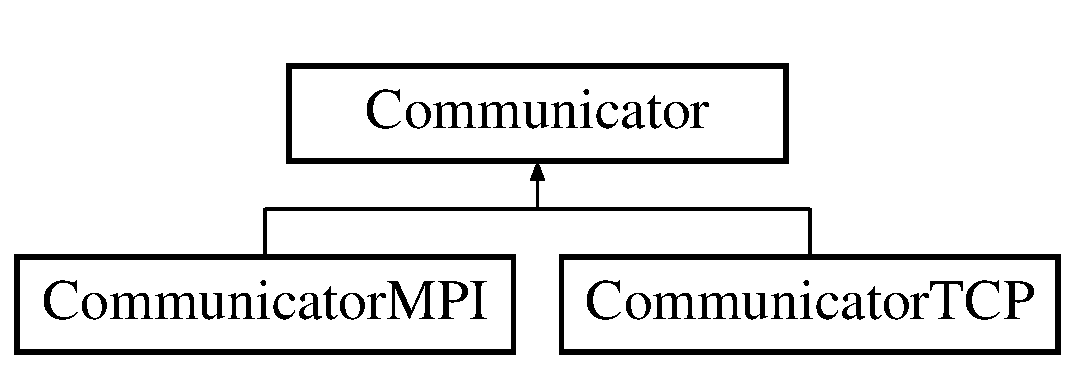
\includegraphics[height=2.000000cm]{classCommunicator}
\end{center}
\end{figure}
\subsection*{Public Member Functions}
\begin{DoxyCompactItemize}
\item 
\hypertarget{classCommunicator_a92ad155222aeafd1e5b1bd129809c2e9}{{\bfseries Communicator} (int type\-\_\-)}\label{classCommunicator_a92ad155222aeafd1e5b1bd129809c2e9}

\item 
\hypertarget{classCommunicator_a0a90cca12dcfb5721e9ac334e79c8802}{virtual int {\bfseries send} (const char $\ast$buf, int count, M\-D\-I\-\_\-\-Datatype datatype)=0}\label{classCommunicator_a0a90cca12dcfb5721e9ac334e79c8802}

\item 
\hypertarget{classCommunicator_af8618383684b7f2e1cea1a40acd43a81}{virtual int {\bfseries recv} (char $\ast$buf, int count, M\-D\-I\-\_\-\-Datatype datatype)=0}\label{classCommunicator_af8618383684b7f2e1cea1a40acd43a81}

\end{DoxyCompactItemize}


The documentation for this class was generated from the following files\-:\begin{DoxyCompactItemize}
\item 
/home/tbarnes/mdi/molssi\-\_\-driver\-\_\-interface/molssi\-\_\-driver\-\_\-interface/\hyperlink{communicator_8h}{communicator.\-h}\item 
/home/tbarnes/mdi/molssi\-\_\-driver\-\_\-interface/molssi\-\_\-driver\-\_\-interface/\hyperlink{communicator_8cpp}{communicator.\-cpp}\end{DoxyCompactItemize}

\hypertarget{classCommunicatorMPI}{\section{Communicator\-M\-P\-I Class Reference}
\label{classCommunicatorMPI}\index{Communicator\-M\-P\-I@{Communicator\-M\-P\-I}}
}
Inheritance diagram for Communicator\-M\-P\-I\-:\begin{figure}[H]
\begin{center}
\leavevmode
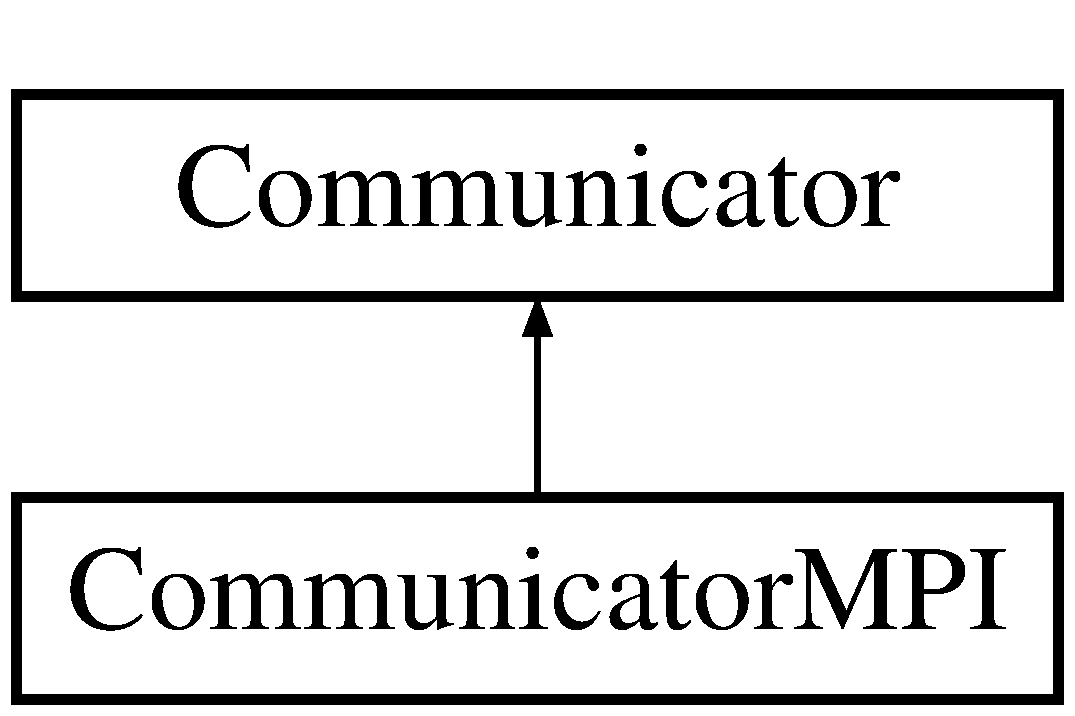
\includegraphics[height=2.000000cm]{classCommunicatorMPI}
\end{center}
\end{figure}
\subsection*{Public Member Functions}
\begin{DoxyCompactItemize}
\item 
\hypertarget{classCommunicatorMPI_aa07167a7e2dcebc0c9050ce1c18f3f32}{{\bfseries Communicator\-M\-P\-I} (int type\-\_\-, int mpi\-\_\-comm\-\_\-, int mpi\-\_\-rank\-\_\-)}\label{classCommunicatorMPI_aa07167a7e2dcebc0c9050ce1c18f3f32}

\item 
\hypertarget{classCommunicatorMPI_afd20883bec05ee4a5d97154a731a13cb}{int {\bfseries send} (const char $\ast$buf, int count, M\-D\-I\-\_\-\-Datatype datatype)}\label{classCommunicatorMPI_afd20883bec05ee4a5d97154a731a13cb}

\item 
\hypertarget{classCommunicatorMPI_ab0852541ca8f78fd3fc32e167386d76d}{int {\bfseries recv} (char $\ast$buf, int count, M\-D\-I\-\_\-\-Datatype datatype)}\label{classCommunicatorMPI_ab0852541ca8f78fd3fc32e167386d76d}

\end{DoxyCompactItemize}


The documentation for this class was generated from the following files\-:\begin{DoxyCompactItemize}
\item 
/home/tbarnes/mdi/molssi\-\_\-driver\-\_\-interface/molssi\-\_\-driver\-\_\-interface/\hyperlink{communicator_8h}{communicator.\-h}\item 
/home/tbarnes/mdi/molssi\-\_\-driver\-\_\-interface/molssi\-\_\-driver\-\_\-interface/\hyperlink{communicator_8cpp}{communicator.\-cpp}\end{DoxyCompactItemize}

\hypertarget{classCommunicatorTCP}{\section{Communicator\-T\-C\-P Class Reference}
\label{classCommunicatorTCP}\index{Communicator\-T\-C\-P@{Communicator\-T\-C\-P}}
}
Inheritance diagram for Communicator\-T\-C\-P\-:\begin{figure}[H]
\begin{center}
\leavevmode
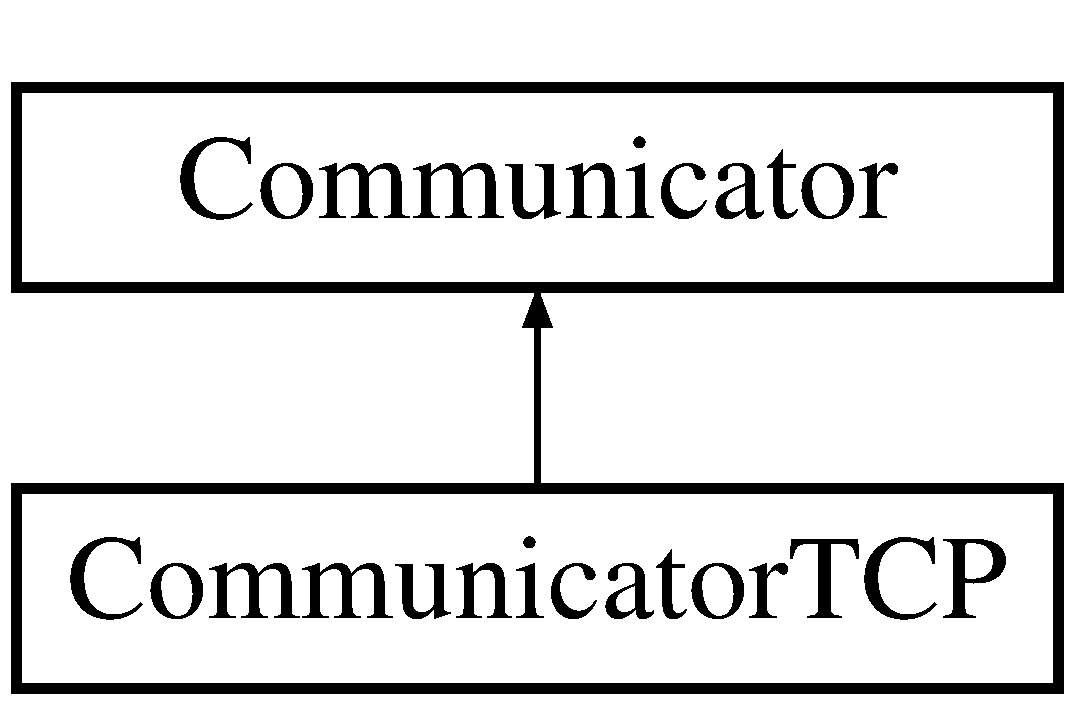
\includegraphics[height=2.000000cm]{classCommunicatorTCP}
\end{center}
\end{figure}
\subsection*{Public Member Functions}
\begin{DoxyCompactItemize}
\item 
\hypertarget{classCommunicatorTCP_a62b8536c01d0e5d3c7ab38df98a9a873}{{\bfseries Communicator\-T\-C\-P} (int type\-\_\-, int sockfd\-\_\-)}\label{classCommunicatorTCP_a62b8536c01d0e5d3c7ab38df98a9a873}

\item 
\hypertarget{classCommunicatorTCP_ac8e4894a12e34596ec7e78ab875933bf}{int {\bfseries send} (const char $\ast$buf, int count, M\-D\-I\-\_\-\-Datatype datatype)}\label{classCommunicatorTCP_ac8e4894a12e34596ec7e78ab875933bf}

\item 
\hypertarget{classCommunicatorTCP_a69d90c24e7bee5736c634565bdebab0d}{int {\bfseries recv} (char $\ast$buf, int count, M\-D\-I\-\_\-\-Datatype datatype)}\label{classCommunicatorTCP_a69d90c24e7bee5736c634565bdebab0d}

\end{DoxyCompactItemize}


The documentation for this class was generated from the following files\-:\begin{DoxyCompactItemize}
\item 
/home/tbarnes/mdi/molssi\-\_\-driver\-\_\-interface/molssi\-\_\-driver\-\_\-interface/\hyperlink{communicator_8h}{communicator.\-h}\item 
/home/tbarnes/mdi/molssi\-\_\-driver\-\_\-interface/molssi\-\_\-driver\-\_\-interface/\hyperlink{communicator_8cpp}{communicator.\-cpp}\end{DoxyCompactItemize}

\hypertarget{classmdi}{\section{mdi Module Reference}
\label{classmdi}\index{mdi@{mdi}}
}
\subsection*{Data Types}
\begin{DoxyCompactItemize}
\item 
interface \hyperlink{interfacemdi_1_1MDI__Accept__Connection__}{M\-D\-I\-\_\-\-Accept\-\_\-\-Connection\-\_\-}
\item 
interface \hyperlink{interfacemdi_1_1MDI__Listen__}{M\-D\-I\-\_\-\-Listen\-\_\-}
\item 
interface \hyperlink{interfacemdi_1_1MDI__MPI__Comm__}{M\-D\-I\-\_\-\-M\-P\-I\-\_\-\-Comm\-\_\-}
\item 
interface \hyperlink{interfacemdi_1_1mdi__recv}{mdi\-\_\-recv}
\item 
interface \hyperlink{interfacemdi_1_1MDI__Recv__}{M\-D\-I\-\_\-\-Recv\-\_\-}
\item 
interface \hyperlink{interfacemdi_1_1MDI__Recv__Command__}{M\-D\-I\-\_\-\-Recv\-\_\-\-Command\-\_\-}
\item 
interface \hyperlink{interfacemdi_1_1MDI__Request__Connection__}{M\-D\-I\-\_\-\-Request\-\_\-\-Connection\-\_\-}
\item 
interface \hyperlink{interfacemdi_1_1mdi__send}{mdi\-\_\-send}
\item 
interface \hyperlink{interfacemdi_1_1MDI__Send__}{M\-D\-I\-\_\-\-Send\-\_\-}
\item 
interface \hyperlink{interfacemdi_1_1MDI__Send__Command__}{M\-D\-I\-\_\-\-Send\-\_\-\-Command\-\_\-}
\end{DoxyCompactItemize}
\subsection*{Public Member Functions}
\begin{DoxyCompactItemize}
\item 
\hypertarget{classmdi_abb29b2ed5c592d2c5e4585ca14ae9c69}{subroutine {\bfseries mdi\-\_\-listen} (fmethod, options, fworld\-\_\-comm, ierr)}\label{classmdi_abb29b2ed5c592d2c5e4585ca14ae9c69}

\item 
\hypertarget{classmdi_ae6b39060c3cc856f240b5239a87a63d8}{subroutine {\bfseries mdi\-\_\-request\-\_\-connection} (fmethod, foptions, fworld\-\_\-comm, comm)}\label{classmdi_ae6b39060c3cc856f240b5239a87a63d8}

\item 
\hypertarget{classmdi_a5f9df9a8c58f50163196ee7ce57d63d6}{subroutine {\bfseries mdi\-\_\-accept\-\_\-connection} (connection)}\label{classmdi_a5f9df9a8c58f50163196ee7ce57d63d6}

\item 
\hypertarget{classmdi_a127a7303cd7217c0d0d646e10b188f39}{subroutine {\bfseries mdi\-\_\-mpi\-\_\-comm} (comm, ierr)}\label{classmdi_a127a7303cd7217c0d0d646e10b188f39}

\item 
\hypertarget{classmdi_a83a8409162740c37f82776526e19d4cf}{subroutine {\bfseries mdi\-\_\-send\-\_\-s} (fstring, len, type, sockfd, ierr)}\label{classmdi_a83a8409162740c37f82776526e19d4cf}

\item 
\hypertarget{classmdi_ad5a7755632e8712b6d5609e2486b184a}{subroutine {\bfseries mdi\-\_\-send\-\_\-d} (fdata, len, type, sockfd, ierr)}\label{classmdi_ad5a7755632e8712b6d5609e2486b184a}

\item 
\hypertarget{classmdi_a57bcbe45a8445f19b02126f904b43774}{subroutine {\bfseries mdi\-\_\-send\-\_\-dv} (fdata, len, type, sockfd, ierr)}\label{classmdi_a57bcbe45a8445f19b02126f904b43774}

\item 
\hypertarget{classmdi_a9451f9ead8226273424cb7efbef245c3}{subroutine {\bfseries mdi\-\_\-send\-\_\-i} (fdata, len, type, sockfd, ierr)}\label{classmdi_a9451f9ead8226273424cb7efbef245c3}

\item 
\hypertarget{classmdi_add16db0836d8e0f3cfe310e175e8243c}{subroutine {\bfseries mdi\-\_\-send\-\_\-iv} (fdata, len, type, sockfd, ierr)}\label{classmdi_add16db0836d8e0f3cfe310e175e8243c}

\item 
\hypertarget{classmdi_a78af4fc262563d2d8820a3a7cbfe0a92}{subroutine {\bfseries mdi\-\_\-recv\-\_\-s} (fstring, len, type, sockfd, ierr)}\label{classmdi_a78af4fc262563d2d8820a3a7cbfe0a92}

\item 
\hypertarget{classmdi_a557c30482625b71f46ee392d70426014}{subroutine {\bfseries mdi\-\_\-recv\-\_\-d} (fdata, len, type, sockfd, ierr)}\label{classmdi_a557c30482625b71f46ee392d70426014}

\item 
\hypertarget{classmdi_a66dc1c9e1462e5c53bd36c720aa12a38}{subroutine {\bfseries mdi\-\_\-recv\-\_\-dv} (fdata, len, type, sockfd, ierr)}\label{classmdi_a66dc1c9e1462e5c53bd36c720aa12a38}

\item 
\hypertarget{classmdi_a50204266766bbd60ec46f697309b9c5c}{subroutine {\bfseries mdi\-\_\-recv\-\_\-i} (fdata, len, type, sockfd, ierr)}\label{classmdi_a50204266766bbd60ec46f697309b9c5c}

\item 
\hypertarget{classmdi_adb59292b64be533922c3bd55c04df653}{subroutine {\bfseries mdi\-\_\-recv\-\_\-iv} (fdata, len, type, sockfd, ierr)}\label{classmdi_adb59292b64be533922c3bd55c04df653}

\item 
\hypertarget{classmdi_a9b4dc2e960271e8779e842b9e1edc0dd}{subroutine {\bfseries mdi\-\_\-send\-\_\-command} (fstring, sockfd, ierr)}\label{classmdi_a9b4dc2e960271e8779e842b9e1edc0dd}

\item 
\hypertarget{classmdi_a3a3b366cde72e01a9d3a928e902e58d0}{subroutine {\bfseries mdi\-\_\-recv\-\_\-command} (fstring, sockfd, ierr)}\label{classmdi_a3a3b366cde72e01a9d3a928e902e58d0}

\end{DoxyCompactItemize}
\subsection*{Public Attributes}
\begin{DoxyCompactItemize}
\item 
\hypertarget{classmdi_accae5b01e087f8738d86006e68417f6d}{integer, dimension(c, name=\char`\"{}mdi\-\_\-kelvin\-\_\-to\-\_\-hartree\char`\"{}), \\*
protected {\bfseries bind}}\label{classmdi_accae5b01e087f8738d86006e68417f6d}

\item 
\hypertarget{classmdi_a476a171077b89b7bc1e0153edaee118a}{integer, protected {\bfseries mdi\-\_\-command\-\_\-length}}\label{classmdi_a476a171077b89b7bc1e0153edaee118a}

\item 
\hypertarget{classmdi_a8038fa45863d082fafb692e8bc1f4b5a}{integer, protected {\bfseries mdi\-\_\-name\-\_\-length}}\label{classmdi_a8038fa45863d082fafb692e8bc1f4b5a}

\item 
\hypertarget{classmdi_ae85ef43174229bd688543ad4bcc08a2b}{integer, protected {\bfseries mdi\-\_\-int}}\label{classmdi_ae85ef43174229bd688543ad4bcc08a2b}

\item 
\hypertarget{classmdi_a69ba399f9ad46c8ac033b26574c9b6ef}{integer, protected {\bfseries mdi\-\_\-double}}\label{classmdi_a69ba399f9ad46c8ac033b26574c9b6ef}

\item 
\hypertarget{classmdi_a5741adbde5b79f06a9b94b17c7f16eb7}{integer, protected {\bfseries mdi\-\_\-char}}\label{classmdi_a5741adbde5b79f06a9b94b17c7f16eb7}

\item 
\hypertarget{classmdi_a1605c457efb88fc7e1f169734c58b52c}{integer, protected {\bfseries mdi\-\_\-tcp}}\label{classmdi_a1605c457efb88fc7e1f169734c58b52c}

\item 
\hypertarget{classmdi_a4039d7ab89098798e98dda20ece81eaf}{integer, protected {\bfseries mdi\-\_\-mpi}}\label{classmdi_a4039d7ab89098798e98dda20ece81eaf}

\item 
\hypertarget{classmdi_aff013df9c91a218d860486ff0fc757e4}{real(kind=8), dimension(c, \\*
name=\char`\"{}mdi\-\_\-kelvin\-\_\-to\-\_\-hartree\char`\"{}), \\*
protected {\bfseries bind}}\label{classmdi_aff013df9c91a218d860486ff0fc757e4}

\item 
\hypertarget{classmdi_af74f78803c251e23cd5022a8df7abc1e}{real(kind=8), protected {\bfseries mdi\-\_\-meter\-\_\-to\-\_\-bohr}}\label{classmdi_af74f78803c251e23cd5022a8df7abc1e}

\item 
\hypertarget{classmdi_a6abac217d729188855210e9327333578}{real(kind=8), protected {\bfseries mdi\-\_\-angstrom\-\_\-to\-\_\-bohr}}\label{classmdi_a6abac217d729188855210e9327333578}

\item 
\hypertarget{classmdi_a583e3421719bbf0bd951f455a0032766}{real(kind=8), protected {\bfseries mdi\-\_\-second\-\_\-to\-\_\-aut}}\label{classmdi_a583e3421719bbf0bd951f455a0032766}

\item 
\hypertarget{classmdi_ad350838a7aea84b6eca15da72d3ee4fc}{real(kind=8), protected {\bfseries mdi\-\_\-picosecond\-\_\-to\-\_\-aut}}\label{classmdi_ad350838a7aea84b6eca15da72d3ee4fc}

\item 
\hypertarget{classmdi_ace10d5db76cf54244d54b62e77b9d9a6}{real(kind=8), protected {\bfseries mdi\-\_\-newton\-\_\-to\-\_\-auf}}\label{classmdi_ace10d5db76cf54244d54b62e77b9d9a6}

\item 
\hypertarget{classmdi_a0b4e777d36fe90d506f70b16abb1b910}{real(kind=8), protected {\bfseries mdi\-\_\-joule\-\_\-to\-\_\-hartree}}\label{classmdi_a0b4e777d36fe90d506f70b16abb1b910}

\item 
\hypertarget{classmdi_a12a5c4e648f84d60dd261349d5e2cf37}{real(kind=8), protected {\bfseries mdi\-\_\-kj\-\_\-to\-\_\-hartree}}\label{classmdi_a12a5c4e648f84d60dd261349d5e2cf37}

\item 
\hypertarget{classmdi_a761336e719b236672a145cf86a8b7c95}{real(kind=8), protected {\bfseries mdi\-\_\-kjpermol\-\_\-to\-\_\-hartree}}\label{classmdi_a761336e719b236672a145cf86a8b7c95}

\item 
\hypertarget{classmdi_a2a5635f450c619dabb104846fd972b22}{real(kind=8), protected {\bfseries mdi\-\_\-kcalpermol\-\_\-to\-\_\-hartree}}\label{classmdi_a2a5635f450c619dabb104846fd972b22}

\item 
\hypertarget{classmdi_a02fe8f5658dc9d6379ceb2cc40b24b56}{real(kind=8), protected {\bfseries mdi\-\_\-ev\-\_\-to\-\_\-hartree}}\label{classmdi_a02fe8f5658dc9d6379ceb2cc40b24b56}

\item 
\hypertarget{classmdi_a4eefaa8b0fe9c708b1ba69ae86bac95c}{real(kind=8), protected {\bfseries mdi\-\_\-rydberg\-\_\-to\-\_\-hartree}}\label{classmdi_a4eefaa8b0fe9c708b1ba69ae86bac95c}

\item 
\hypertarget{classmdi_a5fc09af33b0b858f96014b3f9fdd7ee5}{real(kind=8), protected {\bfseries mdi\-\_\-kelvin\-\_\-to\-\_\-hartree}}\label{classmdi_a5fc09af33b0b858f96014b3f9fdd7ee5}

\end{DoxyCompactItemize}


The documentation for this module was generated from the following file\-:\begin{DoxyCompactItemize}
\item 
/home/tbarnes/mdi/molssi\-\_\-driver\-\_\-interface/molssi\-\_\-driver\-\_\-interface/mdi\-\_\-f90.\-f90\end{DoxyCompactItemize}

\hypertarget{interfacemdi_1_1MDI__Accept__Communicator__}{}\doxysection{mdi\+::M\+D\+I\+\_\+\+Accept\+\_\+\+Communicator\+\_\+ Interface Reference}
\label{interfacemdi_1_1MDI__Accept__Communicator__}\index{mdi::MDI\_Accept\_Communicator\_@{mdi::MDI\_Accept\_Communicator\_}}
\doxysubsection*{Public Member Functions}
\begin{DoxyCompactItemize}
\item 
\mbox{\Hypertarget{interfacemdi_1_1MDI__Accept__Communicator___af692624300292e68edf192a9379e4182}\label{interfacemdi_1_1MDI__Accept__Communicator___af692624300292e68edf192a9379e4182}} 
integer(kind=c\+\_\+int) function {\bfseries mdi\+\_\+accept\+\_\+communicator\+\_\+} ()
\end{DoxyCompactItemize}


The documentation for this interface was generated from the following file\+:\begin{DoxyCompactItemize}
\item 
/\+Users/tbarnes/\+Documents/mdi/molssi\+\_\+driver\+\_\+interface/molssi\+\_\+driver\+\_\+interface/mdi\+\_\+f90.\+f90\end{DoxyCompactItemize}

\hypertarget{interfacemdi_1_1MDI__Conversion__Factor__}{\section{mdi\-:\-:M\-D\-I\-\_\-\-Conversion\-\_\-\-Factor\-\_\- Interface Reference}
\label{interfacemdi_1_1MDI__Conversion__Factor__}\index{mdi\-::\-M\-D\-I\-\_\-\-Conversion\-\_\-\-Factor\-\_\-@{mdi\-::\-M\-D\-I\-\_\-\-Conversion\-\_\-\-Factor\-\_\-}}
}
\subsection*{Public Member Functions}
\begin{DoxyCompactItemize}
\item 
\hypertarget{interfacemdi_1_1MDI__Conversion__Factor___acad6a9822471076622182f03b6073c77}{real(kind=c\-\_\-double) function {\bfseries mdi\-\_\-conversion\-\_\-factor\-\_\-} (in\-\_\-unit, out\-\_\-unit)}\label{interfacemdi_1_1MDI__Conversion__Factor___acad6a9822471076622182f03b6073c77}

\end{DoxyCompactItemize}


The documentation for this interface was generated from the following file\-:\begin{DoxyCompactItemize}
\item 
/home/tbarnes/mdi/molssi\-\_\-driver\-\_\-interface/molssi\-\_\-driver\-\_\-interface/mdi\-\_\-f90.\-f90\end{DoxyCompactItemize}

\hypertarget{interfacemdi_1_1MDI__Init__}{\section{mdi\-:\-:M\-D\-I\-\_\-\-Init\-\_\- Interface Reference}
\label{interfacemdi_1_1MDI__Init__}\index{mdi\-::\-M\-D\-I\-\_\-\-Init\-\_\-@{mdi\-::\-M\-D\-I\-\_\-\-Init\-\_\-}}
}
\subsection*{Public Member Functions}
\begin{DoxyCompactItemize}
\item 
\hypertarget{interfacemdi_1_1MDI__Init___a6d3a67f8175464baa0a4e54caecfa2ae}{integer(kind=c\-\_\-int) function {\bfseries mdi\-\_\-init\-\_\-} (options, world\-\_\-comm)}\label{interfacemdi_1_1MDI__Init___a6d3a67f8175464baa0a4e54caecfa2ae}

\end{DoxyCompactItemize}


The documentation for this interface was generated from the following file\-:\begin{DoxyCompactItemize}
\item 
/home/tbarnes/mdi/molssi\-\_\-driver\-\_\-interface/molssi\-\_\-driver\-\_\-interface/mdi\-\_\-f90.\-f90\end{DoxyCompactItemize}

\hypertarget{interfacemdi_1_1mdi__recv}{\section{mdi\-:\-:mdi\-\_\-recv Interface Reference}
\label{interfacemdi_1_1mdi__recv}\index{mdi\-::mdi\-\_\-recv@{mdi\-::mdi\-\_\-recv}}
}
\subsection*{Public Member Functions}
\begin{DoxyCompactItemize}
\item 
\hypertarget{interfacemdi_1_1mdi__recv_afe159c297131305b07194ea277b8bcdd}{subroutine {\bfseries mdi\-\_\-recv\-\_\-s} (fstring, len, type, sockfd, ierr)}\label{interfacemdi_1_1mdi__recv_afe159c297131305b07194ea277b8bcdd}

\item 
\hypertarget{interfacemdi_1_1mdi__recv_ac75517b0c538096fe258fde546b25d1f}{subroutine {\bfseries mdi\-\_\-recv\-\_\-d} (fdata, len, type, sockfd, ierr)}\label{interfacemdi_1_1mdi__recv_ac75517b0c538096fe258fde546b25d1f}

\item 
\hypertarget{interfacemdi_1_1mdi__recv_ab9cc46f4ff0b31d86b44b93f72330ae8}{subroutine {\bfseries mdi\-\_\-recv\-\_\-dv} (fdata, len, type, sockfd, ierr)}\label{interfacemdi_1_1mdi__recv_ab9cc46f4ff0b31d86b44b93f72330ae8}

\item 
\hypertarget{interfacemdi_1_1mdi__recv_ab7174c24f6e240b8863cb4f41dfb297a}{subroutine {\bfseries mdi\-\_\-recv\-\_\-i} (fdata, len, type, sockfd, ierr)}\label{interfacemdi_1_1mdi__recv_ab7174c24f6e240b8863cb4f41dfb297a}

\item 
\hypertarget{interfacemdi_1_1mdi__recv_abf3328c1bad78a2141268c7ef5707613}{subroutine {\bfseries mdi\-\_\-recv\-\_\-iv} (fdata, len, type, sockfd, ierr)}\label{interfacemdi_1_1mdi__recv_abf3328c1bad78a2141268c7ef5707613}

\end{DoxyCompactItemize}


The documentation for this interface was generated from the following file\-:\begin{DoxyCompactItemize}
\item 
/home/tbarnes/mdi/molssi\-\_\-driver\-\_\-interface/molssi\-\_\-driver\-\_\-interface/mdi\-\_\-f90.\-f90\end{DoxyCompactItemize}

\hypertarget{interfacemdi_1_1MDI__Recv__}{\section{mdi\-:\-:M\-D\-I\-\_\-\-Recv\-\_\- Interface Reference}
\label{interfacemdi_1_1MDI__Recv__}\index{mdi\-::\-M\-D\-I\-\_\-\-Recv\-\_\-@{mdi\-::\-M\-D\-I\-\_\-\-Recv\-\_\-}}
}
\subsection*{Public Member Functions}
\begin{DoxyCompactItemize}
\item 
\hypertarget{interfacemdi_1_1MDI__Recv___a8a02f4e2009b1219ed101b4b2c2584ed}{integer(kind=c\-\_\-int) function {\bfseries mdi\-\_\-recv\-\_\-} (buf, count, datatype, comm)}\label{interfacemdi_1_1MDI__Recv___a8a02f4e2009b1219ed101b4b2c2584ed}

\end{DoxyCompactItemize}


The documentation for this interface was generated from the following file\-:\begin{DoxyCompactItemize}
\item 
/home/tbarnes/mdi/molssi\-\_\-driver\-\_\-interface/molssi\-\_\-driver\-\_\-interface/mdi\-\_\-f90.\-f90\end{DoxyCompactItemize}

\hypertarget{interfacemdi_1_1MDI__Recv__Command__}{\section{mdi\-:\-:M\-D\-I\-\_\-\-Recv\-\_\-\-Command\-\_\- Interface Reference}
\label{interfacemdi_1_1MDI__Recv__Command__}\index{mdi\-::\-M\-D\-I\-\_\-\-Recv\-\_\-\-Command\-\_\-@{mdi\-::\-M\-D\-I\-\_\-\-Recv\-\_\-\-Command\-\_\-}}
}
\subsection*{Public Member Functions}
\begin{DoxyCompactItemize}
\item 
\hypertarget{interfacemdi_1_1MDI__Recv__Command___a22b67734eebe9ccf72cd71a8894c28e4}{integer(kind=c\-\_\-int) function {\bfseries mdi\-\_\-recv\-\_\-command\-\_\-} (buf, comm)}\label{interfacemdi_1_1MDI__Recv__Command___a22b67734eebe9ccf72cd71a8894c28e4}

\end{DoxyCompactItemize}


The documentation for this interface was generated from the following file\-:\begin{DoxyCompactItemize}
\item 
/home/tbarnes/mdi/molssi\-\_\-driver\-\_\-interface/molssi\-\_\-driver\-\_\-interface/mdi\-\_\-f90.\-f90\end{DoxyCompactItemize}

\hypertarget{interfacemdi_1_1mdi__send}{}\doxysection{mdi\+::mdi\+\_\+send Interface Reference}
\label{interfacemdi_1_1mdi__send}\index{mdi::mdi\_send@{mdi::mdi\_send}}
\doxysubsection*{Public Member Functions}
\begin{DoxyCompactItemize}
\item 
\mbox{\Hypertarget{interfacemdi_1_1mdi__send_abd109b0b0e0b3f95e9782cf01d8ab7bb}\label{interfacemdi_1_1mdi__send_abd109b0b0e0b3f95e9782cf01d8ab7bb}} 
subroutine {\bfseries mdi\+\_\+send\+\_\+s} (fbuf, count, datatype, comm, ierr)
\item 
\mbox{\Hypertarget{interfacemdi_1_1mdi__send_a609eb3114aba823f801636fc4013165c}\label{interfacemdi_1_1mdi__send_a609eb3114aba823f801636fc4013165c}} 
subroutine {\bfseries mdi\+\_\+send\+\_\+d} (fbuf, count, datatype, comm, ierr)
\item 
\mbox{\Hypertarget{interfacemdi_1_1mdi__send_a891088c993f8f958c97ab01f4a504a42}\label{interfacemdi_1_1mdi__send_a891088c993f8f958c97ab01f4a504a42}} 
subroutine {\bfseries mdi\+\_\+send\+\_\+dv} (fbuf, count, datatype, comm, ierr)
\item 
\mbox{\Hypertarget{interfacemdi_1_1mdi__send_ab11c98611174127b27f723aef2055f64}\label{interfacemdi_1_1mdi__send_ab11c98611174127b27f723aef2055f64}} 
subroutine {\bfseries mdi\+\_\+send\+\_\+i} (fbuf, count, datatype, comm, ierr)
\item 
\mbox{\Hypertarget{interfacemdi_1_1mdi__send_a2890417bf9b36440044e97ddfb3a448c}\label{interfacemdi_1_1mdi__send_a2890417bf9b36440044e97ddfb3a448c}} 
subroutine {\bfseries mdi\+\_\+send\+\_\+iv} (fbuf, count, datatype, comm, ierr)
\end{DoxyCompactItemize}


The documentation for this interface was generated from the following file\+:\begin{DoxyCompactItemize}
\item 
/\+Users/tbarnes/\+Documents/mdi/molssi\+\_\+driver\+\_\+interface/molssi\+\_\+driver\+\_\+interface/mdi\+\_\+f90.\+f90\end{DoxyCompactItemize}

\hypertarget{interfacemdi_1_1MDI__Send__}{\section{mdi\-:\-:M\-D\-I\-\_\-\-Send\-\_\- Interface Reference}
\label{interfacemdi_1_1MDI__Send__}\index{mdi\-::\-M\-D\-I\-\_\-\-Send\-\_\-@{mdi\-::\-M\-D\-I\-\_\-\-Send\-\_\-}}
}
\subsection*{Public Member Functions}
\begin{DoxyCompactItemize}
\item 
\hypertarget{interfacemdi_1_1MDI__Send___a696dd7ff266143903df4669aca92d32f}{integer(kind=c\-\_\-int) function {\bfseries mdi\-\_\-send\-\_\-} (data\-\_\-ptr, len, type, sockfd)}\label{interfacemdi_1_1MDI__Send___a696dd7ff266143903df4669aca92d32f}

\end{DoxyCompactItemize}


The documentation for this interface was generated from the following file\-:\begin{DoxyCompactItemize}
\item 
/home/tbarnes/mdi/molssi\-\_\-driver\-\_\-interface/molssi\-\_\-driver\-\_\-interface/mdi\-\_\-f90.\-f90\end{DoxyCompactItemize}

\hypertarget{interfacemdi_1_1MDI__Send__Command__}{\section{mdi\-:\-:M\-D\-I\-\_\-\-Send\-\_\-\-Command\-\_\- Interface Reference}
\label{interfacemdi_1_1MDI__Send__Command__}\index{mdi\-::\-M\-D\-I\-\_\-\-Send\-\_\-\-Command\-\_\-@{mdi\-::\-M\-D\-I\-\_\-\-Send\-\_\-\-Command\-\_\-}}
}
\subsection*{Public Member Functions}
\begin{DoxyCompactItemize}
\item 
\hypertarget{interfacemdi_1_1MDI__Send__Command___ad79374503988a8b76342367a2b38feb5}{integer(kind=c\-\_\-int) function {\bfseries mdi\-\_\-send\-\_\-command\-\_\-} (buf, comm)}\label{interfacemdi_1_1MDI__Send__Command___ad79374503988a8b76342367a2b38feb5}

\end{DoxyCompactItemize}


The documentation for this interface was generated from the following file\-:\begin{DoxyCompactItemize}
\item 
/home/tbarnes/mdi/molssi\-\_\-driver\-\_\-interface/molssi\-\_\-driver\-\_\-interface/mdi\-\_\-f90.\-f90\end{DoxyCompactItemize}

\hypertarget{classMDIManager}{\section{M\-D\-I\-Manager Class Reference}
\label{classMDIManager}\index{M\-D\-I\-Manager@{M\-D\-I\-Manager}}
}
\subsection*{Public Member Functions}
\begin{DoxyCompactItemize}
\item 
\hypertarget{classMDIManager_a7d02f65b6ec14d2b94f30309fc297725}{{\bfseries M\-D\-I\-Manager} (const char $\ast$options, void $\ast$world\-\_\-comm)}\label{classMDIManager_a7d02f65b6ec14d2b94f30309fc297725}

\item 
\hypertarget{classMDIManager_aead8acfd8e9328b845015a8ba1b1ac01}{int {\bfseries accept\-\_\-communicator} ()}\label{classMDIManager_aead8acfd8e9328b845015a8ba1b1ac01}

\item 
\hypertarget{classMDIManager_acbd50272ac3d42086be3981c6107adc8}{int {\bfseries send} (const char $\ast$buf, int count, M\-D\-I\-\_\-\-Datatype datatype, M\-D\-I\-\_\-\-Comm comm)}\label{classMDIManager_acbd50272ac3d42086be3981c6107adc8}

\item 
\hypertarget{classMDIManager_a8a6caab0db63267bf117e44253943de9}{int {\bfseries recv} (char $\ast$buf, int count, M\-D\-I\-\_\-\-Datatype datatype, M\-D\-I\-\_\-\-Comm comm)}\label{classMDIManager_a8a6caab0db63267bf117e44253943de9}

\item 
\hypertarget{classMDIManager_ab154bc23f32381088e89848deac2f701}{int {\bfseries send\-\_\-command} (const char $\ast$buf, M\-D\-I\-\_\-\-Comm comm)}\label{classMDIManager_ab154bc23f32381088e89848deac2f701}

\item 
\hypertarget{classMDIManager_a0689b1d5ee97d5936c760dc8f6418ef4}{int {\bfseries recv\-\_\-command} (char $\ast$buf, M\-D\-I\-\_\-\-Comm comm)}\label{classMDIManager_a0689b1d5ee97d5936c760dc8f6418ef4}

\end{DoxyCompactItemize}
\subsection*{Public Attributes}
\begin{DoxyCompactItemize}
\item 
\hypertarget{classMDIManager_a81f7d832fd9e1fd6168874dcdcaf2ad1}{\hyperlink{classMethodTCP}{Method\-T\-C\-P} $\ast$ {\bfseries method\-\_\-tcp}}\label{classMDIManager_a81f7d832fd9e1fd6168874dcdcaf2ad1}

\item 
\hypertarget{classMDIManager_a7b320b241377c1a356245dbd2a3bc707}{\hyperlink{classMethodMPI}{Method\-M\-P\-I} $\ast$ {\bfseries method\-\_\-mpi}}\label{classMDIManager_a7b320b241377c1a356245dbd2a3bc707}

\end{DoxyCompactItemize}


The documentation for this class was generated from the following files\-:\begin{DoxyCompactItemize}
\item 
/home/tbarnes/mdi/molssi\-\_\-driver\-\_\-interface/molssi\-\_\-driver\-\_\-interface/\hyperlink{mdi__manager_8h}{mdi\-\_\-manager.\-h}\item 
/home/tbarnes/mdi/molssi\-\_\-driver\-\_\-interface/molssi\-\_\-driver\-\_\-interface/\hyperlink{mdi__manager_8cpp}{mdi\-\_\-manager.\-cpp}\end{DoxyCompactItemize}

\hypertarget{classMethodMPI}{\section{Method\-M\-P\-I Class Reference}
\label{classMethodMPI}\index{Method\-M\-P\-I@{Method\-M\-P\-I}}
}
\subsection*{Public Member Functions}
\begin{DoxyCompactItemize}
\item 
\hypertarget{classMethodMPI_ad1c0de09adc11a28665ff79c8a8c0204}{int {\bfseries gather\-\_\-names} (const char $\ast$hostname\-\_\-ptr, bool do\-\_\-split)}\label{classMethodMPI_ad1c0de09adc11a28665ff79c8a8c0204}

\item 
\hypertarget{classMethodMPI_ac6eb460a524a9fe7e36e6a14eabc2c4a}{int {\bfseries split\-\_\-mpi\-\_\-communicator} (void $\ast$world\-\_\-comm)}\label{classMethodMPI_ac6eb460a524a9fe7e36e6a14eabc2c4a}

\end{DoxyCompactItemize}
\subsection*{Public Attributes}
\begin{DoxyCompactItemize}
\item 
\hypertarget{classMethodMPI_a9d6daa11fdd9246e8c1eea2cb0376162}{M\-P\-I\-\_\-\-Comm {\bfseries intra\-\_\-\-M\-P\-I\-\_\-comm}}\label{classMethodMPI_a9d6daa11fdd9246e8c1eea2cb0376162}

\item 
\hypertarget{classMethodMPI_a01db6ba3138f94147b56ab34bcec4f66}{int {\bfseries intra\-\_\-rank}}\label{classMethodMPI_a01db6ba3138f94147b56ab34bcec4f66}

\item 
\hypertarget{classMethodMPI_a089003d4d1c9b32d8f7a7a67cd544a80}{int {\bfseries mpi\-\_\-code\-\_\-rank}}\label{classMethodMPI_a089003d4d1c9b32d8f7a7a67cd544a80}

\end{DoxyCompactItemize}


The documentation for this class was generated from the following files\-:\begin{DoxyCompactItemize}
\item 
/home/tbarnes/mdi/molssi\-\_\-driver\-\_\-interface/molssi\-\_\-driver\-\_\-interface/\hyperlink{method_8h}{method.\-h}\item 
/home/tbarnes/mdi/molssi\-\_\-driver\-\_\-interface/molssi\-\_\-driver\-\_\-interface/\hyperlink{method_8cpp}{method.\-cpp}\end{DoxyCompactItemize}

\hypertarget{classMethodTCP}{\section{Method\-T\-C\-P Class Reference}
\label{classMethodTCP}\index{Method\-T\-C\-P@{Method\-T\-C\-P}}
}
\subsection*{Public Member Functions}
\begin{DoxyCompactItemize}
\item 
\hypertarget{classMethodTCP_ac57708cf27dc538f3545e831147f84a9}{int {\bfseries M\-D\-I\-\_\-\-Listen\-\_\-\-T\-C\-P} (int port)}\label{classMethodTCP_ac57708cf27dc538f3545e831147f84a9}

\item 
\hypertarget{classMethodTCP_a5e3e9cf897c337db7149d857e7457278}{int {\bfseries M\-D\-I\-\_\-\-Request\-\_\-\-Connection\-\_\-\-T\-C\-P} (int port, char $\ast$hostname\-\_\-ptr)}\label{classMethodTCP_a5e3e9cf897c337db7149d857e7457278}

\item 
\hypertarget{classMethodTCP_a2c66a5df73ca84946a949b76cbd97908}{int {\bfseries On\-\_\-\-Accept\-\_\-\-Communicator} ()}\label{classMethodTCP_a2c66a5df73ca84946a949b76cbd97908}

\end{DoxyCompactItemize}
\subsection*{Public Attributes}
\begin{DoxyCompactItemize}
\item 
\hypertarget{classMethodTCP_ae89fa007b11d6a3e97200d1f4d5033b4}{int {\bfseries tcp\-\_\-socket}}\label{classMethodTCP_ae89fa007b11d6a3e97200d1f4d5033b4}

\end{DoxyCompactItemize}


The documentation for this class was generated from the following files\-:\begin{DoxyCompactItemize}
\item 
/home/tbarnes/mdi/molssi\-\_\-driver\-\_\-interface/molssi\-\_\-driver\-\_\-interface/\hyperlink{method_8h}{method.\-h}\item 
/home/tbarnes/mdi/molssi\-\_\-driver\-\_\-interface/molssi\-\_\-driver\-\_\-interface/\hyperlink{method_8cpp}{method.\-cpp}\end{DoxyCompactItemize}

\chapter{File Documentation}
\hypertarget{communicator_8cpp}{\section{/home/tbarnes/mdi/molssi\-\_\-driver\-\_\-interface/molssi\-\_\-driver\-\_\-interface/communicator.cpp File Reference}
\label{communicator_8cpp}\index{/home/tbarnes/mdi/molssi\-\_\-driver\-\_\-interface/molssi\-\_\-driver\-\_\-interface/communicator.\-cpp@{/home/tbarnes/mdi/molssi\-\_\-driver\-\_\-interface/molssi\-\_\-driver\-\_\-interface/communicator.\-cpp}}
}


Class definition for handling communication between connect codes.  


{\ttfamily \#include $<$mpi.\-h$>$}\\*
{\ttfamily \#include $<$stdio.\-h$>$}\\*
{\ttfamily \#include $<$stdlib.\-h$>$}\\*
{\ttfamily \#include $<$unistd.\-h$>$}\\*
{\ttfamily \#include \char`\"{}mdi.\-h\char`\"{}}\\*
{\ttfamily \#include \char`\"{}communicator.\-h\char`\"{}}\\*
\subsection*{Variables}
\begin{DoxyCompactItemize}
\item 
\hypertarget{communicator_8cpp_a1806a2b57b24b2dd653eb4475758e5d2}{vector$<$ \hyperlink{classCommunicator}{Communicator} $\ast$ $>$ {\bfseries communicators}}\label{communicator_8cpp_a1806a2b57b24b2dd653eb4475758e5d2}

\end{DoxyCompactItemize}


\subsection{Detailed Description}
Class definition for handling communication between connect codes. 
\hypertarget{communicator_8h}{\section{/home/tbarnes/mdi/molssi\-\_\-driver\-\_\-interface/molssi\-\_\-driver\-\_\-interface/communicator.h File Reference}
\label{communicator_8h}\index{/home/tbarnes/mdi/molssi\-\_\-driver\-\_\-interface/molssi\-\_\-driver\-\_\-interface/communicator.\-h@{/home/tbarnes/mdi/molssi\-\_\-driver\-\_\-interface/molssi\-\_\-driver\-\_\-interface/communicator.\-h}}
}


Class declaration for handling communication between connected codes.  


{\ttfamily \#include $<$vector$>$}\\*
{\ttfamily \#include \char`\"{}mdi.\-h\char`\"{}}\\*
\subsection*{Classes}
\begin{DoxyCompactItemize}
\item 
class \hyperlink{classCommunicator}{Communicator}
\item 
class \hyperlink{classCommunicatorMPI}{Communicator\-M\-P\-I}
\item 
class \hyperlink{classCommunicatorTCP}{Communicator\-T\-C\-P}
\end{DoxyCompactItemize}
\subsection*{Variables}
\begin{DoxyCompactItemize}
\item 
\hypertarget{communicator_8h_a7e67b3696ce162a35e70e0b87e093caf}{std\-::vector$<$ \hyperlink{classCommunicator}{Communicator} $\ast$ $>$ {\bfseries communicators}}\label{communicator_8h_a7e67b3696ce162a35e70e0b87e093caf}

\end{DoxyCompactItemize}


\subsection{Detailed Description}
Class declaration for handling communication between connected codes. 
\hypertarget{mdi_8cpp}{\section{/home/tbarnes/mdi/molssi\-\_\-driver\-\_\-interface/molssi\-\_\-driver\-\_\-interface/mdi.cpp File Reference}
\label{mdi_8cpp}\index{/home/tbarnes/mdi/molssi\-\_\-driver\-\_\-interface/molssi\-\_\-driver\-\_\-interface/mdi.\-cpp@{/home/tbarnes/mdi/molssi\-\_\-driver\-\_\-interface/molssi\-\_\-driver\-\_\-interface/mdi.\-cpp}}
}


Functions callable by users of the Mol\-S\-S\-I Driver Interface.  


{\ttfamily \#include $<$signal.\-h$>$}\\*
{\ttfamily \#include $<$netdb.\-h$>$}\\*
{\ttfamily \#include $<$netinet/in.\-h$>$}\\*
{\ttfamily \#include $<$stdio.\-h$>$}\\*
{\ttfamily \#include $<$stdlib.\-h$>$}\\*
{\ttfamily \#include $<$string.\-h$>$}\\*
{\ttfamily \#include $<$sys/socket.\-h$>$}\\*
{\ttfamily \#include $<$sys/types.\-h$>$}\\*
{\ttfamily \#include $<$sys/un.\-h$>$}\\*
{\ttfamily \#include $<$unistd.\-h$>$}\\*
{\ttfamily \#include $<$errno.\-h$>$}\\*
{\ttfamily \#include $<$iostream$>$}\\*
{\ttfamily \#include $<$vector$>$}\\*
{\ttfamily \#include \char`\"{}mdi.\-h\char`\"{}}\\*
{\ttfamily \#include \char`\"{}communicator.\-h\char`\"{}}\\*
{\ttfamily \#include \char`\"{}mdi\-\_\-manager.\-h\char`\"{}}\\*
{\ttfamily \#include \char`\"{}method.\-h\char`\"{}}\\*
\subsection*{Functions}
\begin{DoxyCompactItemize}
\item 
\hypertarget{mdi_8cpp_a10ceefc902b8eb71e2383d7ac95de2c7}{void {\bfseries mdi\-\_\-error} (const char $\ast$message)}\label{mdi_8cpp_a10ceefc902b8eb71e2383d7ac95de2c7}

\item 
int \hyperlink{mdi_8cpp_ae05ae377fa8de592f62c696c041b7d0a}{M\-D\-I\-\_\-\-Init} (const char $\ast$options, void $\ast$world\-\_\-comm)
\begin{DoxyCompactList}\small\item\em Initialize communication through the M\-D\-I library. \end{DoxyCompactList}\item 
M\-D\-I\-\_\-\-Comm \hyperlink{mdi_8cpp_a570557fdd42049c5e285faf546037531}{M\-D\-I\-\_\-\-Accept\-\_\-\-Communicator} ()
\begin{DoxyCompactList}\small\item\em Accept a new M\-D\-I communicator. \end{DoxyCompactList}\item 
int \hyperlink{mdi_8cpp_a5356b5fe5aca86c3390e13f8762a01e1}{M\-D\-I\-\_\-\-Send} (const char $\ast$buf, int count, M\-D\-I\-\_\-\-Datatype datatype, M\-D\-I\-\_\-\-Comm comm)
\begin{DoxyCompactList}\small\item\em Send data through the M\-D\-I connection. \end{DoxyCompactList}\item 
int \hyperlink{mdi_8cpp_ac94ed31fb09c8445b40265a89c72e006}{M\-D\-I\-\_\-\-Recv} (char $\ast$buf, int count, M\-D\-I\-\_\-\-Datatype datatype, M\-D\-I\-\_\-\-Comm comm)
\begin{DoxyCompactList}\small\item\em Receive data through the M\-D\-I connection. \end{DoxyCompactList}\item 
int \hyperlink{mdi_8cpp_a77e579331a36c3f0eb7f7ff9668e789d}{M\-D\-I\-\_\-\-Send\-\_\-\-Command} (const char $\ast$buf, M\-D\-I\-\_\-\-Comm comm)
\begin{DoxyCompactList}\small\item\em Send a command of length {\ttfamily M\-D\-I\-\_\-\-C\-O\-M\-M\-A\-N\-D\-\_\-\-L\-E\-N\-G\-T\-H} through the M\-D\-I connection. \end{DoxyCompactList}\item 
int \hyperlink{mdi_8cpp_ab03c0ea8beda690d6f796d3089cbfe15}{M\-D\-I\-\_\-\-Recv\-\_\-\-Command} (char $\ast$buf, M\-D\-I\-\_\-\-Comm comm)
\begin{DoxyCompactList}\small\item\em Receive a command of length {\ttfamily M\-D\-I\-\_\-\-C\-O\-M\-M\-A\-N\-D\-\_\-\-L\-E\-N\-G\-T\-H} through the M\-D\-I connection. \end{DoxyCompactList}\item 
double \hyperlink{mdi_8cpp_a886c1af1124f55d869a6f2b80a68c5a7}{M\-D\-I\-\_\-\-Conversion\-\_\-\-Factor} (char $\ast$in\-\_\-unit, char $\ast$out\-\_\-unit)
\begin{DoxyCompactList}\small\item\em Return a conversion factor between two units. \end{DoxyCompactList}\item 
\hypertarget{mdi_8cpp_a0accde4a79728e8eaab73632daba3c15}{int {\bfseries M\-D\-I\-\_\-\-Get\-\_\-\-M\-P\-I\-\_\-\-Code\-\_\-\-Rank} ()}\label{mdi_8cpp_a0accde4a79728e8eaab73632daba3c15}

\item 
\hypertarget{mdi_8cpp_a6290edc0924c7f9375e4cb9e0c7a7744}{void {\bfseries M\-D\-I\-\_\-\-Set\-\_\-\-M\-P\-I\-\_\-\-Intra\-\_\-\-Rank} (int rank)}\label{mdi_8cpp_a6290edc0924c7f9375e4cb9e0c7a7744}

\end{DoxyCompactItemize}
\subsection*{Variables}
\begin{DoxyCompactItemize}
\item 
\hypertarget{mdi_8cpp_ae5fcebdb64c7844358e07e880bcb15c2}{const int {\bfseries M\-D\-I\-\_\-\-C\-O\-M\-M\-A\-N\-D\-\_\-\-L\-E\-N\-G\-T\-H} = 12}\label{mdi_8cpp_ae5fcebdb64c7844358e07e880bcb15c2}

\item 
\hypertarget{mdi_8cpp_a8ca47e903a62de4298767ef3d446901d}{const int {\bfseries M\-D\-I\-\_\-\-N\-A\-M\-E\-\_\-\-L\-E\-N\-G\-T\-H} = 12}\label{mdi_8cpp_a8ca47e903a62de4298767ef3d446901d}

\item 
\hypertarget{mdi_8cpp_a96172c3cbab16d7b9e80288a7c94f241}{const M\-D\-I\-\_\-\-Comm {\bfseries M\-D\-I\-\_\-\-N\-U\-L\-L\-\_\-\-C\-O\-M\-M} = 0}\label{mdi_8cpp_a96172c3cbab16d7b9e80288a7c94f241}

\item 
\hypertarget{mdi_8cpp_ab88e0bb1563ba9fa73ffc49a704e43ad}{const int {\bfseries M\-D\-I\-\_\-\-I\-N\-T} = 0}\label{mdi_8cpp_ab88e0bb1563ba9fa73ffc49a704e43ad}

\item 
\hypertarget{mdi_8cpp_a3d0c16831c941e5b870461394bfe5c82}{const int {\bfseries M\-D\-I\-\_\-\-D\-O\-U\-B\-L\-E} = 1}\label{mdi_8cpp_a3d0c16831c941e5b870461394bfe5c82}

\item 
\hypertarget{mdi_8cpp_a508f568d6a6cba24d6015347d6c1469e}{const int {\bfseries M\-D\-I\-\_\-\-C\-H\-A\-R} = 2}\label{mdi_8cpp_a508f568d6a6cba24d6015347d6c1469e}

\item 
\hypertarget{mdi_8cpp_a1be671d11b9e0779a06a79abeceadd39}{const int {\bfseries M\-D\-I\-\_\-\-I\-N\-T\-\_\-\-N\-U\-M\-P\-Y} = 3}\label{mdi_8cpp_a1be671d11b9e0779a06a79abeceadd39}

\item 
\hypertarget{mdi_8cpp_aaf7153f9eda53a820f81f59ddb484ced}{const int {\bfseries M\-D\-I\-\_\-\-D\-O\-U\-B\-L\-E\-\_\-\-N\-U\-M\-P\-Y} = 4}\label{mdi_8cpp_aaf7153f9eda53a820f81f59ddb484ced}

\item 
\hypertarget{mdi_8cpp_aa69d77aeaab908058636a4420b02ae90}{const int {\bfseries M\-D\-I\-\_\-\-T\-C\-P} = 1}\label{mdi_8cpp_aa69d77aeaab908058636a4420b02ae90}

\item 
\hypertarget{mdi_8cpp_ac9eaa23189e2bf8a92c2136ee0112a87}{const int {\bfseries M\-D\-I\-\_\-\-M\-P\-I} = 2}\label{mdi_8cpp_ac9eaa23189e2bf8a92c2136ee0112a87}

\item 
\hypertarget{mdi_8cpp_a323937b5877ef054dc40e584ef767070}{const double {\bfseries M\-D\-I\-\_\-\-M\-E\-T\-E\-R\-\_\-\-T\-O\-\_\-\-B\-O\-H\-R} = 1.\-88972612546e10}\label{mdi_8cpp_a323937b5877ef054dc40e584ef767070}

\item 
\hypertarget{mdi_8cpp_ad7fb89aef0dfdc7caffe72d45b7d01d7}{const double {\bfseries M\-D\-I\-\_\-\-A\-N\-G\-S\-T\-R\-O\-M\-\_\-\-T\-O\-\_\-\-B\-O\-H\-R} = 1.\-88972612546}\label{mdi_8cpp_ad7fb89aef0dfdc7caffe72d45b7d01d7}

\item 
\hypertarget{mdi_8cpp_a9a119f46a44d6d6f594d44c8b897f9e8}{const double {\bfseries M\-D\-I\-\_\-\-S\-E\-C\-O\-N\-D\-\_\-\-T\-O\-\_\-\-A\-U\-T} = 4.\-1341374575751e16}\label{mdi_8cpp_a9a119f46a44d6d6f594d44c8b897f9e8}

\item 
\hypertarget{mdi_8cpp_a191439a37d783bcfd2c4e4989b5b2cde}{const double {\bfseries M\-D\-I\-\_\-\-P\-I\-C\-O\-S\-E\-C\-O\-N\-D\-\_\-\-T\-O\-\_\-\-A\-U\-T} = 4.\-1341374575751e4}\label{mdi_8cpp_a191439a37d783bcfd2c4e4989b5b2cde}

\item 
\hypertarget{mdi_8cpp_a3d051436cb3d2b9b9fb8528ecc70f1e6}{const double {\bfseries M\-D\-I\-\_\-\-N\-E\-W\-T\-O\-N\-\_\-\-T\-O\-\_\-\-A\-U\-F} = 1.\-213780478e7}\label{mdi_8cpp_a3d051436cb3d2b9b9fb8528ecc70f1e6}

\item 
\hypertarget{mdi_8cpp_ae40c10c77dccde242ad259fd26fd3619}{const double {\bfseries M\-D\-I\-\_\-\-J\-O\-U\-L\-E\-\_\-\-T\-O\-\_\-\-H\-A\-R\-T\-R\-E\-E} = 2.\-29371265835792e17}\label{mdi_8cpp_ae40c10c77dccde242ad259fd26fd3619}

\item 
\hypertarget{mdi_8cpp_a61e9917a12f86564edf9ef812d92fa4a}{const double {\bfseries M\-D\-I\-\_\-\-K\-J\-\_\-\-T\-O\-\_\-\-H\-A\-R\-T\-R\-E\-E} = 2.\-29371265835792e20}\label{mdi_8cpp_a61e9917a12f86564edf9ef812d92fa4a}

\item 
\hypertarget{mdi_8cpp_a27ea253093fdfdad5592091fe1f62870}{const double {\bfseries M\-D\-I\-\_\-\-K\-J\-P\-E\-R\-M\-O\-L\-\_\-\-T\-O\-\_\-\-H\-A\-R\-T\-R\-E\-E} = 3.\-80879947807451e-\/4}\label{mdi_8cpp_a27ea253093fdfdad5592091fe1f62870}

\item 
\hypertarget{mdi_8cpp_ae4f6e7e76d00e3222ec87ab235388435}{const double {\bfseries M\-D\-I\-\_\-\-K\-C\-A\-L\-P\-E\-R\-M\-O\-L\-\_\-\-T\-O\-\_\-\-H\-A\-R\-T\-R\-E\-E} = 1.\-5941730215480900e-\/3}\label{mdi_8cpp_ae4f6e7e76d00e3222ec87ab235388435}

\item 
\hypertarget{mdi_8cpp_ad50c706a104210c0c9d38ad2ee3b47dd}{const double {\bfseries M\-D\-I\-\_\-\-E\-V\-\_\-\-T\-O\-\_\-\-H\-A\-R\-T\-R\-E\-E} = 3.\-67493266806491e-\/2}\label{mdi_8cpp_ad50c706a104210c0c9d38ad2ee3b47dd}

\item 
\hypertarget{mdi_8cpp_a87b24c6eb5745296de8723de5cb7208d}{const double {\bfseries M\-D\-I\-\_\-\-R\-Y\-D\-B\-E\-R\-G\-\_\-\-T\-O\-\_\-\-H\-A\-R\-T\-R\-E\-E} = 0.\-5}\label{mdi_8cpp_a87b24c6eb5745296de8723de5cb7208d}

\item 
\hypertarget{mdi_8cpp_a40cfa9151564f12c5a0ebbee1697381e}{const double {\bfseries M\-D\-I\-\_\-\-K\-E\-L\-V\-I\-N\-\_\-\-T\-O\-\_\-\-H\-A\-R\-T\-R\-E\-E} = 3.\-16681050847798e-\/6}\label{mdi_8cpp_a40cfa9151564f12c5a0ebbee1697381e}

\end{DoxyCompactItemize}


\subsection{Detailed Description}
Functions callable by users of the Mol\-S\-S\-I Driver Interface. 

\subsection{Function Documentation}
\hypertarget{mdi_8cpp_a570557fdd42049c5e285faf546037531}{\index{mdi.\-cpp@{mdi.\-cpp}!M\-D\-I\-\_\-\-Accept\-\_\-\-Communicator@{M\-D\-I\-\_\-\-Accept\-\_\-\-Communicator}}
\index{M\-D\-I\-\_\-\-Accept\-\_\-\-Communicator@{M\-D\-I\-\_\-\-Accept\-\_\-\-Communicator}!mdi.cpp@{mdi.\-cpp}}
\subsubsection[{M\-D\-I\-\_\-\-Accept\-\_\-\-Communicator}]{\setlength{\rightskip}{0pt plus 5cm}M\-D\-I\-\_\-\-Comm M\-D\-I\-\_\-\-Accept\-\_\-\-Communicator (
\begin{DoxyParamCaption}
{}
\end{DoxyParamCaption}
)}}\label{mdi_8cpp_a570557fdd42049c5e285faf546037531}


Accept a new M\-D\-I communicator. 

The function returns an M\-D\-I\-\_\-\-Comm that describes a connection between two codes. If no new communicators are available, the function returns {\ttfamily M\-D\-I\-\_\-\-N\-U\-L\-L\-\_\-\-C\-O\-M\-M}. \hypertarget{mdi_8cpp_a886c1af1124f55d869a6f2b80a68c5a7}{\index{mdi.\-cpp@{mdi.\-cpp}!M\-D\-I\-\_\-\-Conversion\-\_\-\-Factor@{M\-D\-I\-\_\-\-Conversion\-\_\-\-Factor}}
\index{M\-D\-I\-\_\-\-Conversion\-\_\-\-Factor@{M\-D\-I\-\_\-\-Conversion\-\_\-\-Factor}!mdi.cpp@{mdi.\-cpp}}
\subsubsection[{M\-D\-I\-\_\-\-Conversion\-\_\-\-Factor}]{\setlength{\rightskip}{0pt plus 5cm}double M\-D\-I\-\_\-\-Conversion\-\_\-\-Factor (
\begin{DoxyParamCaption}
\item[{char $\ast$}]{in\-\_\-unit, }
\item[{char $\ast$}]{out\-\_\-unit}
\end{DoxyParamCaption}
)}}\label{mdi_8cpp_a886c1af1124f55d869a6f2b80a68c5a7}


Return a conversion factor between two units. 

The function returns the conversion factor from {\ttfamily in\-\_\-unit} to {\ttfamily out\-\_\-unit}.


\begin{DoxyParams}[1]{Parameters}
\mbox{\tt in}  & {\em in\-\_\-unit} & Name of the unit to convert from. \\
\hline
\mbox{\tt in}  & {\em out\-\_\-unit} & Name of the unit to convert to. \\
\hline
\end{DoxyParams}
\hypertarget{mdi_8cpp_ae05ae377fa8de592f62c696c041b7d0a}{\index{mdi.\-cpp@{mdi.\-cpp}!M\-D\-I\-\_\-\-Init@{M\-D\-I\-\_\-\-Init}}
\index{M\-D\-I\-\_\-\-Init@{M\-D\-I\-\_\-\-Init}!mdi.cpp@{mdi.\-cpp}}
\subsubsection[{M\-D\-I\-\_\-\-Init}]{\setlength{\rightskip}{0pt plus 5cm}int M\-D\-I\-\_\-\-Init (
\begin{DoxyParamCaption}
\item[{const char $\ast$}]{options, }
\item[{void $\ast$}]{world\-\_\-comm}
\end{DoxyParamCaption}
)}}\label{mdi_8cpp_ae05ae377fa8de592f62c696c041b7d0a}


Initialize communication through the M\-D\-I library. 

If using the \char`\"{}-\/method M\-P\-I\char`\"{} option, this function must be called by all ranks. The function returns {\ttfamily 0} on a success.


\begin{DoxyParams}[1]{Parameters}
\mbox{\tt in}  & {\em options} & Options describing the communication method used to connect to codes \\
\hline
\mbox{\tt in,out}  & {\em world\-\_\-comm} & On input, the M\-P\-I communicator that spans all of the codes. On output, the M\-P\-I communicator that spans the single code corresponding to the calling rank. Only used if the \char`\"{}-\/method M\-P\-I\char`\"{} option is provided. \\
\hline
\end{DoxyParams}
\hypertarget{mdi_8cpp_ac94ed31fb09c8445b40265a89c72e006}{\index{mdi.\-cpp@{mdi.\-cpp}!M\-D\-I\-\_\-\-Recv@{M\-D\-I\-\_\-\-Recv}}
\index{M\-D\-I\-\_\-\-Recv@{M\-D\-I\-\_\-\-Recv}!mdi.cpp@{mdi.\-cpp}}
\subsubsection[{M\-D\-I\-\_\-\-Recv}]{\setlength{\rightskip}{0pt plus 5cm}int M\-D\-I\-\_\-\-Recv (
\begin{DoxyParamCaption}
\item[{char $\ast$}]{buf, }
\item[{int}]{count, }
\item[{M\-D\-I\-\_\-\-Datatype}]{datatype, }
\item[{M\-D\-I\-\_\-\-Comm}]{comm}
\end{DoxyParamCaption}
)}}\label{mdi_8cpp_ac94ed31fb09c8445b40265a89c72e006}


Receive data through the M\-D\-I connection. 

If running with M\-P\-I, this function must be called only by rank {\ttfamily 0}. The function returns {\ttfamily 0} on a success.


\begin{DoxyParams}[1]{Parameters}
\mbox{\tt in}  & {\em buf} & Pointer to the buffer where the received data will be stored. \\
\hline
\mbox{\tt in}  & {\em count} & Number of values (integers, double precision floats, characters, etc.) to be received. \\
\hline
\mbox{\tt in}  & {\em datatype} & M\-D\-I handle (M\-D\-I\-\_\-\-I\-N\-T, M\-D\-I\-\_\-\-D\-O\-U\-B\-L\-E, M\-D\-I\-\_\-\-C\-H\-A\-R, etc.) corresponding to the type of data to be received. \\
\hline
\mbox{\tt in}  & {\em comm} & M\-D\-I communicator associated with the connection to the sending code. \\
\hline
\end{DoxyParams}
\hypertarget{mdi_8cpp_ab03c0ea8beda690d6f796d3089cbfe15}{\index{mdi.\-cpp@{mdi.\-cpp}!M\-D\-I\-\_\-\-Recv\-\_\-\-Command@{M\-D\-I\-\_\-\-Recv\-\_\-\-Command}}
\index{M\-D\-I\-\_\-\-Recv\-\_\-\-Command@{M\-D\-I\-\_\-\-Recv\-\_\-\-Command}!mdi.cpp@{mdi.\-cpp}}
\subsubsection[{M\-D\-I\-\_\-\-Recv\-\_\-\-Command}]{\setlength{\rightskip}{0pt plus 5cm}int M\-D\-I\-\_\-\-Recv\-\_\-\-Command (
\begin{DoxyParamCaption}
\item[{char $\ast$}]{buf, }
\item[{M\-D\-I\-\_\-\-Comm}]{comm}
\end{DoxyParamCaption}
)}}\label{mdi_8cpp_ab03c0ea8beda690d6f796d3089cbfe15}


Receive a command of length {\ttfamily M\-D\-I\-\_\-\-C\-O\-M\-M\-A\-N\-D\-\_\-\-L\-E\-N\-G\-T\-H} through the M\-D\-I connection. 

If running with M\-P\-I, this function must be called only by rank {\ttfamily 0}. The function returns {\ttfamily 0} on a success.


\begin{DoxyParams}[1]{Parameters}
\mbox{\tt in}  & {\em buf} & Pointer to the buffer where the received data will be stored. \\
\hline
\mbox{\tt in}  & {\em comm} & M\-D\-I communicator associated with the connection to the sending code. \\
\hline
\end{DoxyParams}
\hypertarget{mdi_8cpp_a5356b5fe5aca86c3390e13f8762a01e1}{\index{mdi.\-cpp@{mdi.\-cpp}!M\-D\-I\-\_\-\-Send@{M\-D\-I\-\_\-\-Send}}
\index{M\-D\-I\-\_\-\-Send@{M\-D\-I\-\_\-\-Send}!mdi.cpp@{mdi.\-cpp}}
\subsubsection[{M\-D\-I\-\_\-\-Send}]{\setlength{\rightskip}{0pt plus 5cm}int M\-D\-I\-\_\-\-Send (
\begin{DoxyParamCaption}
\item[{const char $\ast$}]{buf, }
\item[{int}]{count, }
\item[{M\-D\-I\-\_\-\-Datatype}]{datatype, }
\item[{M\-D\-I\-\_\-\-Comm}]{comm}
\end{DoxyParamCaption}
)}}\label{mdi_8cpp_a5356b5fe5aca86c3390e13f8762a01e1}


Send data through the M\-D\-I connection. 

If running with M\-P\-I, this function must be called only by rank {\ttfamily 0}. The function returns {\ttfamily 0} on a success.


\begin{DoxyParams}[1]{Parameters}
\mbox{\tt in}  & {\em buf} & Pointer to the data to be sent. \\
\hline
\mbox{\tt in}  & {\em count} & Number of values (integers, double precision floats, characters, etc.) to be sent. \\
\hline
\mbox{\tt in}  & {\em datatype} & M\-D\-I handle (M\-D\-I\-\_\-\-I\-N\-T, M\-D\-I\-\_\-\-D\-O\-U\-B\-L\-E, M\-D\-I\-\_\-\-C\-H\-A\-R, etc.) corresponding to the type of data to be sent. \\
\hline
\mbox{\tt in}  & {\em comm} & M\-D\-I communicator associated with the intended recipient code. \\
\hline
\end{DoxyParams}
\hypertarget{mdi_8cpp_a77e579331a36c3f0eb7f7ff9668e789d}{\index{mdi.\-cpp@{mdi.\-cpp}!M\-D\-I\-\_\-\-Send\-\_\-\-Command@{M\-D\-I\-\_\-\-Send\-\_\-\-Command}}
\index{M\-D\-I\-\_\-\-Send\-\_\-\-Command@{M\-D\-I\-\_\-\-Send\-\_\-\-Command}!mdi.cpp@{mdi.\-cpp}}
\subsubsection[{M\-D\-I\-\_\-\-Send\-\_\-\-Command}]{\setlength{\rightskip}{0pt plus 5cm}int M\-D\-I\-\_\-\-Send\-\_\-\-Command (
\begin{DoxyParamCaption}
\item[{const char $\ast$}]{buf, }
\item[{M\-D\-I\-\_\-\-Comm}]{comm}
\end{DoxyParamCaption}
)}}\label{mdi_8cpp_a77e579331a36c3f0eb7f7ff9668e789d}


Send a command of length {\ttfamily M\-D\-I\-\_\-\-C\-O\-M\-M\-A\-N\-D\-\_\-\-L\-E\-N\-G\-T\-H} through the M\-D\-I connection. 

If running with M\-P\-I, this function must be called only by rank {\ttfamily 0}. The function returns {\ttfamily 0} on a success.


\begin{DoxyParams}[1]{Parameters}
\mbox{\tt in}  & {\em buf} & Pointer to the data to be sent. \\
\hline
\mbox{\tt in}  & {\em comm} & M\-D\-I communicator associated with the intended recipient code. \\
\hline
\end{DoxyParams}

\hypertarget{mdi__manager_8cpp}{\section{/home/tbarnes/mdi/molssi\-\_\-driver\-\_\-interface/molssi\-\_\-driver\-\_\-interface/mdi\-\_\-manager.cpp File Reference}
\label{mdi__manager_8cpp}\index{/home/tbarnes/mdi/molssi\-\_\-driver\-\_\-interface/molssi\-\_\-driver\-\_\-interface/mdi\-\_\-manager.\-cpp@{/home/tbarnes/mdi/molssi\-\_\-driver\-\_\-interface/molssi\-\_\-driver\-\_\-interface/mdi\-\_\-manager.\-cpp}}
}


Class definition for top-\/level manager of M\-D\-I operations.  


{\ttfamily \#include $<$mpi.\-h$>$}\\*
{\ttfamily \#include $<$stdio.\-h$>$}\\*
{\ttfamily \#include $<$stdlib.\-h$>$}\\*
{\ttfamily \#include $<$string.\-h$>$}\\*
{\ttfamily \#include $<$unistd.\-h$>$}\\*
{\ttfamily \#include \char`\"{}mdi.\-h\char`\"{}}\\*
{\ttfamily \#include \char`\"{}mdi\-\_\-manager.\-h\char`\"{}}\\*
{\ttfamily \#include \char`\"{}communicator.\-h\char`\"{}}\\*


\subsection{Detailed Description}
Class definition for top-\/level manager of M\-D\-I operations. 
\hypertarget{mdi__manager_8h}{\section{/home/tbarnes/mdi/molssi\-\_\-driver\-\_\-interface/molssi\-\_\-driver\-\_\-interface/mdi\-\_\-manager.h File Reference}
\label{mdi__manager_8h}\index{/home/tbarnes/mdi/molssi\-\_\-driver\-\_\-interface/molssi\-\_\-driver\-\_\-interface/mdi\-\_\-manager.\-h@{/home/tbarnes/mdi/molssi\-\_\-driver\-\_\-interface/molssi\-\_\-driver\-\_\-interface/mdi\-\_\-manager.\-h}}
}


Class declaration for top-\/level manager of M\-D\-I operations.  


{\ttfamily \#include $<$vector$>$}\\*
{\ttfamily \#include \char`\"{}mdi.\-h\char`\"{}}\\*
{\ttfamily \#include \char`\"{}method.\-h\char`\"{}}\\*
\subsection*{Classes}
\begin{DoxyCompactItemize}
\item 
class \hyperlink{classMDIManager}{M\-D\-I\-Manager}
\end{DoxyCompactItemize}


\subsection{Detailed Description}
Class declaration for top-\/level manager of M\-D\-I operations. 
\hypertarget{method_8cpp}{\section{/home/tbarnes/mdi/molssi\-\_\-driver\-\_\-interface/molssi\-\_\-driver\-\_\-interface/method.cpp File Reference}
\label{method_8cpp}\index{/home/tbarnes/mdi/molssi\-\_\-driver\-\_\-interface/molssi\-\_\-driver\-\_\-interface/method.\-cpp@{/home/tbarnes/mdi/molssi\-\_\-driver\-\_\-interface/molssi\-\_\-driver\-\_\-interface/method.\-cpp}}
}


Class definition for top-\/level manager of M\-D\-I operations.  


{\ttfamily \#include $<$mpi.\-h$>$}\\*
{\ttfamily \#include $<$stdio.\-h$>$}\\*
{\ttfamily \#include $<$stdlib.\-h$>$}\\*
{\ttfamily \#include $<$string.\-h$>$}\\*
{\ttfamily \#include $<$unistd.\-h$>$}\\*
{\ttfamily \#include $<$netinet/in.\-h$>$}\\*
{\ttfamily \#include $<$sys/socket.\-h$>$}\\*
{\ttfamily \#include $<$signal.\-h$>$}\\*
{\ttfamily \#include $<$errno.\-h$>$}\\*
{\ttfamily \#include $<$netdb.\-h$>$}\\*
{\ttfamily \#include \char`\"{}mdi.\-h\char`\"{}}\\*
{\ttfamily \#include \char`\"{}method.\-h\char`\"{}}\\*
{\ttfamily \#include \char`\"{}communicator.\-h\char`\"{}}\\*
\subsection*{Functions}
\begin{DoxyCompactItemize}
\item 
\hypertarget{method_8cpp_a47630f8f823b92ad9333c3c5f130cf90}{void {\bfseries sigint\-\_\-handler} (int dummy)}\label{method_8cpp_a47630f8f823b92ad9333c3c5f130cf90}

\end{DoxyCompactItemize}


\subsection{Detailed Description}
Class definition for top-\/level manager of M\-D\-I operations. 
\hypertarget{method_8h}{}\doxysection{/\+Users/tbarnes/\+Documents/mdi/molssi\+\_\+driver\+\_\+interface/molssi\+\_\+driver\+\_\+interface/method.h File Reference}
\label{method_8h}\index{/Users/tbarnes/Documents/mdi/molssi\_driver\_interface/molssi\_driver\_interface/method.h@{/Users/tbarnes/Documents/mdi/molssi\_driver\_interface/molssi\_driver\_interface/method.h}}


Class declaration for top-\/level manager of M\+DI operations.  


{\ttfamily \#include $<$mpi.\+h$>$}\newline
{\ttfamily \#include \char`\"{}mdi.\+h\char`\"{}}\newline
\doxysubsection*{Functions}
\begin{DoxyCompactItemize}
\item 
\mbox{\Hypertarget{method_8h_a47630f8f823b92ad9333c3c5f130cf90}\label{method_8h_a47630f8f823b92ad9333c3c5f130cf90}} 
void {\bfseries sigint\+\_\+handler} (int dummy)
\item 
\mbox{\Hypertarget{method_8h_af15a7354cf37401b3a482614dedbcad9}\label{method_8h_af15a7354cf37401b3a482614dedbcad9}} 
int {\bfseries M\+D\+I\+\_\+\+Listen\+\_\+\+T\+CP} (int port)
\item 
\mbox{\Hypertarget{method_8h_a200d815da834074e8a718519b9f833a6}\label{method_8h_a200d815da834074e8a718519b9f833a6}} 
int {\bfseries M\+D\+I\+\_\+\+Request\+\_\+\+Connection\+\_\+\+T\+CP} (int port, char $\ast$hostname\+\_\+ptr)
\item 
\mbox{\Hypertarget{method_8h_a3a7ddb6846048fedb7a50e24e3e6eb48}\label{method_8h_a3a7ddb6846048fedb7a50e24e3e6eb48}} 
int {\bfseries On\+\_\+\+Accept\+\_\+\+Communicator} ()
\item 
\mbox{\Hypertarget{method_8h_a7015ada5eb2def03e044160eb83cfc65}\label{method_8h_a7015ada5eb2def03e044160eb83cfc65}} 
int {\bfseries gather\+\_\+names} (const char $\ast$hostname\+\_\+ptr, int do\+\_\+split)
\item 
\mbox{\Hypertarget{method_8h_aeaa32341a57ef7dc21775b73813e20cc}\label{method_8h_aeaa32341a57ef7dc21775b73813e20cc}} 
int {\bfseries split\+\_\+mpi\+\_\+communicator} (void $\ast$world\+\_\+comm)
\end{DoxyCompactItemize}
\doxysubsection*{Variables}
\begin{DoxyCompactItemize}
\item 
\mbox{\Hypertarget{method_8h_a58bcdde21e0687d1b5634b673451357a}\label{method_8h_a58bcdde21e0687d1b5634b673451357a}} 
int {\bfseries tcp\+\_\+socket}
\item 
\mbox{\Hypertarget{method_8h_a94117669fa21b6293d144b9f2ec9bc77}\label{method_8h_a94117669fa21b6293d144b9f2ec9bc77}} 
M\+P\+I\+\_\+\+Comm {\bfseries intra\+\_\+\+M\+P\+I\+\_\+comm}
\item 
\mbox{\Hypertarget{method_8h_ac7c9ae008d0383e5a99af93c0c0a741c}\label{method_8h_ac7c9ae008d0383e5a99af93c0c0a741c}} 
int {\bfseries intra\+\_\+rank}
\item 
\mbox{\Hypertarget{method_8h_a6da60e1bcb42aadfd89405b192a82cf4}\label{method_8h_a6da60e1bcb42aadfd89405b192a82cf4}} 
int {\bfseries mpi\+\_\+code\+\_\+rank}
\end{DoxyCompactItemize}


\doxysubsection{Detailed Description}
Class declaration for top-\/level manager of M\+DI operations. 


%--- End generated contents ---

% Index
\newpage
\phantomsection
\addcontentsline{toc}{part}{Index}
\printindex

\end{document}
